\chapter{System Analysis \& Design}

\section{Introduction}
Every great software product begins as a response to a complex challenge. For Kemora, the challenge was building a cohesive, highly interactive travel platform that could seamlessly merge AI itinerary generation, social networking, and rich mapping without buckling under its own weight. Early conceptual prototypes quickly revealed the dangers of tight coupling: UI code tangled with business logic, and backend APIs inextricably bound to database frameworks. 

To overcome these hurdles, this chapter delineates our journey in engineering the architectural design of the Kemora platform. Rather than settling for a monolithic anti-pattern, we intentionally designed a system resilient to future expansion and varying loads. The resulting architecture embraces ASP.NET Core \cite{aspnetcore} for the backend API—anchored by Clean Architecture \cite{cleanarchitecture} principles to protect core domain logic—and Flutter \cite{flutter} for the cross-platform mobile frontend, utilizing the Provider pattern \cite{providerpattern} to conquer state management complexities.

\section{Requirements Specification}

\subsection{Functional Requirements}
Functional requirements define the specific behaviors and functions the system must perform. The core functional requirements for Kemora are:
\begin{itemize}
    \item \textbf{FR1 - User Authentication \& Authorization:} The system must allow users to register, log in (via email/password or Google OAuth), and securely manage their sessions. Authentication is handled via JWT tokens, with support for token refresh, email confirmation, and password reset functionalities.
    \item \textbf{FR2 - Destination Discovery:} The system must display a categorized directory of Egyptian governorates and specific tourist attractions, augmented with images (via Cloudinary) and metadata stored exclusively in the local database, with no on-the-fly Google Places fallback.
    \item \textbf{FR3 - AI Trip Generation:} The system must accept user parameters (duration, budget, preferences) and generate a logically ordered, day-by-day itinerary using an external LLM (via OpenRouter).
    \item \textbf{FR4 - Trip Modification (Custom Roadmap):} Users must be able to view their generated trips on an interactive map, manually add places, remove places, and reorder itinerary items dynamically.
    \item \textbf{FR5 - Social Networking \& Community:} The system must provide a community feed where users can publish posts, attach media, leave comments, and react to content. Posts can be directly linked to user-generated AI trips.
    \item \textbf{FR6 - Gamification Engine:} The system must track user actions and automatically award points and badges (e.g., "AiPioneer", "CityHopper") upon crossing specific thresholds.
\end{itemize}

\subsection{Non-Functional Requirements}
Non-functional requirements specify criteria that judge the operation of the system, guaranteeing stability, security, and high performance.
\begin{itemize}
    \item \textbf{NFR1 - Performance \& Caching:} The backend API must respond to standard data retrieval requests in under 100ms under normal load. AI generation requests should resolve within 15 seconds. To achieve this, the system uses in-memory caching (\texttt{MemoryCacheService}) for frequent queries and caches available LLM models concurrently.
    \item \textbf{NFR2 - Scalability:} The architecture must support stateless scaling. Session state must not be stored in server memory. JWTs ensure that requests can be routed to any backend node behind a load balancer. Thread-safe operations (using \texttt{SemaphoreSlim}) ensure safe initialization of singletons like the OpenRouter model cache under high load.
    \item \textbf{NFR3 - Security Protocols:}
    \begin{itemize}
        \item \textbf{Data Encryption:} All communication is encrypted via TLS 1.2/1.3.
        \item \textbf{Password Hashing:} Passwords are cryptographically hashed using PBKDF2 (the ASP.NET Core Identity default) with a high iteration count.
        \item \textbf{JWT Structure:} JSON Web Tokens are signed using the HMAC-SHA512 algorithm (\texttt{SecurityAlgorithms.HmacSha512Signature}). Tokens contain specific claims (\texttt{NameId}, \texttt{Email}, \texttt{GivenName}, \texttt{Role}) and possess a 7-day expiration time to balance user convenience with security. Refresh tokens are generated as 32-byte cryptographically secure random numbers encoded in Base64.
        \item \textbf{Rate Limiting:} Critical endpoints (e.g., \texttt{AuthController}) are protected against brute-force and DDoS attacks via ASP.NET Core Rate Limiting (using the \texttt{[EnableRateLimiting]} attribute).
    \end{itemize}
    \item \textbf{NFR4 - Maintainability:} The backend strictly adheres to Clean Architecture. The Domain layer is completely independent of external frameworks. Application logic is separated into Services (\texttt{TripService}, \texttt{TripPlannerService}), while external integrations reside in the Infrastructure layer (\texttt{AuthService}, \texttt{OpenRouterAiService}). HTTP routing is confined to the API tier (\texttt{TripsController}, \texttt{AuthController}, \texttt{PlacesController}).
\end{itemize}

\section{System Architecture: The Clean Architecture Journey}
As the Kemora backend grew to encompass AI scheduling, social feeds, and gamification, early iterations suffered from the classic "spaghetti code" dilemma. Business rules were scattered across controllers, and swapping out external services (like the AI provider or storage layer) required rewriting core logic. 

To resolve this, we adopted \textbf{Clean Architecture} \cite{cleanarchitecture}. By inverting the dependencies, we ensured that our core business rules remained isolated and independent of UI, databases, or external APIs. This structural discipline is organized into four concentric layers:

\subsection{Architectural Layers}
\begin{enumerate}
    \item \textbf{Domain Layer (The Core):} At the center of our architecture lies the Domain Layer. It contains the fundamental business entities (\texttt{ApplicationUser}, \texttt{Trip}, \texttt{Place}) and repository interfaces. It has zero dependencies on any other project or framework, guaranteeing that our most critical rules are immune to external technological shifts.
    \item \textbf{Application Layer (Use Cases):} Orchestrating the system's capabilities, this layer houses Data Transfer Objects (DTOs), business service interfaces (\texttt{ITripService}, \texttt{IAiService}), and core business logic (\texttt{TripService}, \texttt{TripPlannerService}). It dictates \textit{what} the system does without caring \textit{how} the data is fetched or saved. To decouple side effects, such as our gamification engine, we utilize an \textbf{event-driven architecture} powered by \textbf{MediatR domain events} \cite{mediatr}. Core user actions emit domain events, which are asynchronously handled to award points and badges without blocking the primary request thread.
    \item \textbf{Infrastructure Layer (External Details):} This layer implements the interfaces defined in the Application layer. Whenever we needed to integrate a new third-party capability, it was confined here. Key implementations include \texttt{TokenService} for JWT handling, \texttt{OpenRouterAiService} for communicating with external LLMs, and \texttt{CloudinaryImageService} for media storage.
    \item \textbf{API Layer (The Delivery Mechanism):} Serving as the entry point to the backend, the API layer exposes RESTful endpoints (e.g., \texttt{AuthController}, \texttt{TripsController}) secured via Bearer authentication. It remains thin, delegating all substantial work to the Application layer. To ensure robustness, API contracts are strictly maintained; all incoming requests undergo rigorous validation using \textbf{FluentValidation} \cite{fluentvalidation}, and exceptions or validation failures are uniformly formatted according to the \textbf{RFC 7807} \cite{rfc7807} standard (Problem Details for HTTP APIs).
\end{enumerate}

\begin{figure}[H]
    \centering
    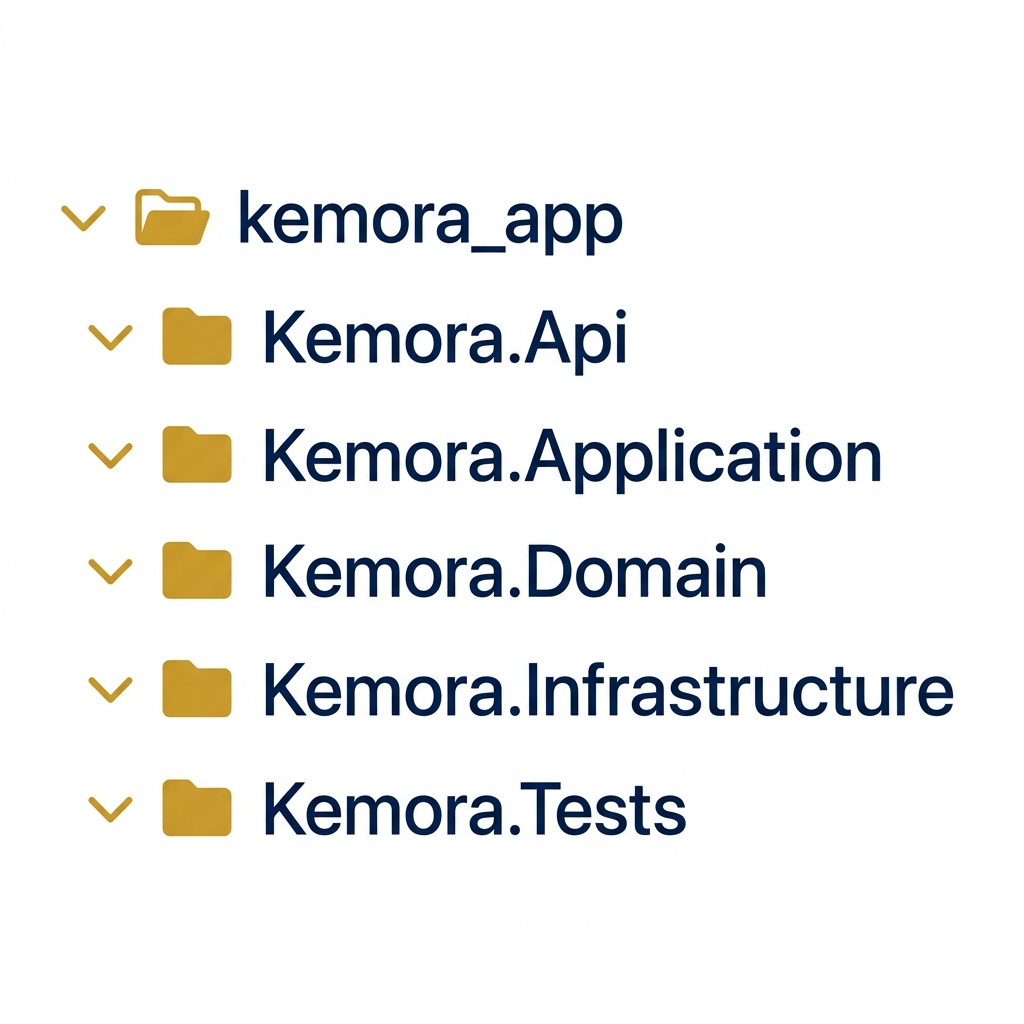
\includegraphics[width=0.9\textwidth]{figures/architecture.png}
    \caption{Kemora's Overall Architecture}
    \label{fig:architecture}
\end{figure}

\subsection{Sequence Diagrams}

\subsubsection{Authentication Flow (JWT Generation)}
The following Mermaid sequence diagram illustrates the login and token generation process when a user authenticates via the \texttt{AuthController}.

\begin{verbatim}
sequenceDiagram
    participant Client as Flutter App
    participant API as AuthController
    participant AuthSvc as AuthService
    participant SignIn as SignInManager
    participant Identity as UserManager
    participant TokenSvc as TokenService
    participant DB as SQL Server

    Client->>API: POST /api/v1/auth/login (email, password)
    API->>AuthSvc: LoginAsync(model)
    AuthSvc->>Identity: FindByEmailAsync(email)
    Identity->>DB: Query User
    DB-->>Identity: Return ApplicationUser
    AuthSvc->>SignIn: CheckPasswordSignInAsync(user, password, false)
    SignIn-->>AuthSvc: Password Valid
    AuthSvc->>TokenSvc: GenerateRefreshToken()
    TokenSvc-->>AuthSvc: Return 32-byte Base64 String
    AuthSvc->>Identity: UpdateAsync(user)
    Identity->>DB: Save Refresh Token to User
    AuthSvc->>TokenSvc: CreateTokenAsync(user)
    TokenSvc->>Identity: GetRolesAsync(user)
    Identity-->>TokenSvc: List of Roles
    Note over TokenSvc: Sign JWT & Attach Claims
    TokenSvc-->>AuthSvc: Return JWT String
    AuthSvc-->>API: Return AuthResponseDto
    API-->>Client: 200 OK (Tokens + User Info)
\end{verbatim}

\subsubsection{AI Trip Generation \& Save Flow}
This diagram outlines the process of requesting an AI-generated itinerary and subsequently saving it to the database using the \texttt{PlacesController}, \texttt{TripsController}, and \texttt{OpenRouterAiService}.

\begin{verbatim}
sequenceDiagram
    participant Client as Flutter App
    participant PlacesAPI as PlacesController
    participant TripsAPI as TripsController
    participant PlannerSvc as TripPlannerService
    participant TripSvc as TripService
    participant AI as OpenRouterAiService
    participant ExtAI as OpenRouter API
    participant Badge as BadgeAwardService
    participant DB as SQL Server

    Client->>PlacesAPI: POST /api/v1/places/trip-plan (TripPlanRequestDto)
    PlacesAPI->>PlannerSvc: GenerateTripPlanAsync(request)
    PlannerSvc->>AI: GenerateCompletionAsync(sysPrompt, userPrompt)
    Note over AI: Check ConcurrentDictionary<br/>for available free models
    AI->>ExtAI: HTTP POST /v1/completions
    ExtAI-->>AI: LLM JSON Response (Itinerary)
    AI-->>PlannerSvc: Parsed TripPlanResponseDto
    PlannerSvc-->>PlacesAPI: Return TripPlanResponseDto
    PlacesAPI-->>Client: 200 OK (Proposed Itinerary)
    
    Note over Client: User reviews and modifies<br/>the itinerary locally
    
    Client->>TripsAPI: POST /api/v1/trips/save-plan (SaveAIPlanDto)
    TripsAPI->>TripSvc: SaveAIPlanAsync(userId, dto)
    TripSvc->>DB: Insert Trip & TripPlaces
    DB-->>TripSvc: Assigned TripID
    TripSvc-->>TripsAPI: Return TripDetailDto
    
    TripsAPI->>Badge: TryAwardAiPioneerAsync(userId)
    Badge->>DB: Check/Update User Badges
    TripsAPI->>Badge: TryAwardCityHopperAsync(userId)
    TripsAPI-->>Client: 201 Created (Trip details)
\end{verbatim}

\subsection{Microservices Readiness \& Bounded Contexts}
Although Kemora is currently deployed as a modular monolith to reduce operational overhead, its architecture is fundamentally designed for a seamless transition to microservices. By strictly adhering to Clean Architecture \cite{cleanarchitecture} and employing MediatR \cite{mediatr} for domain events, the system establishes clear bounded contexts (e.g., Identity, Trip Planning, Social Feed, Gamification). These bounded contexts interact through asynchronous events rather than direct method calls. When the platform scales to a point where independent deployment of these domains becomes necessary, the in-memory MediatR pipelines can easily be replaced with distributed event brokers, such as RabbitMQ \cite{rabbitmq} or Apache Kafka \cite{kafka}, with minimal refactoring of the core business logic.

\section{Database Design and Entity Relationships}
The data tier is powered by a relational SQL Server database schema optimized for entity integrity and rapid querying. The schema is managed via Entity Framework Core \cite{efcore} Code-First migrations.

\subsection{Key Data Entities}
\begin{itemize}
    \item \textbf{ApplicationUser:} Inherits from ASP.NET Identity User. Holds authentication details, accumulated points, and JSON-serialized user preferences.
    \item \textbf{Place \& Governorate:} Hierarchical spatial data. Places are linked to Governorates via foreign keys and are categorized by \texttt{PlaceType}.
    \item \textbf{Trip \& TripPlace:} Represents the AI-generated itineraries. A \texttt{Trip} has a one-to-many relationship with \texttt{TripPlace}, representing the chronological ordering of activities (with precise \texttt{Order} fields for timeline mapping).
    \item \textbf{Post \& Comment:} The core of the social network. Posts link to a \texttt{UserID} and optionally a \texttt{LinkedTripId}, allowing users to seamlessly share their itineraries directly to the feed.
\end{itemize}

\begin{figure}[H]
    \centering
    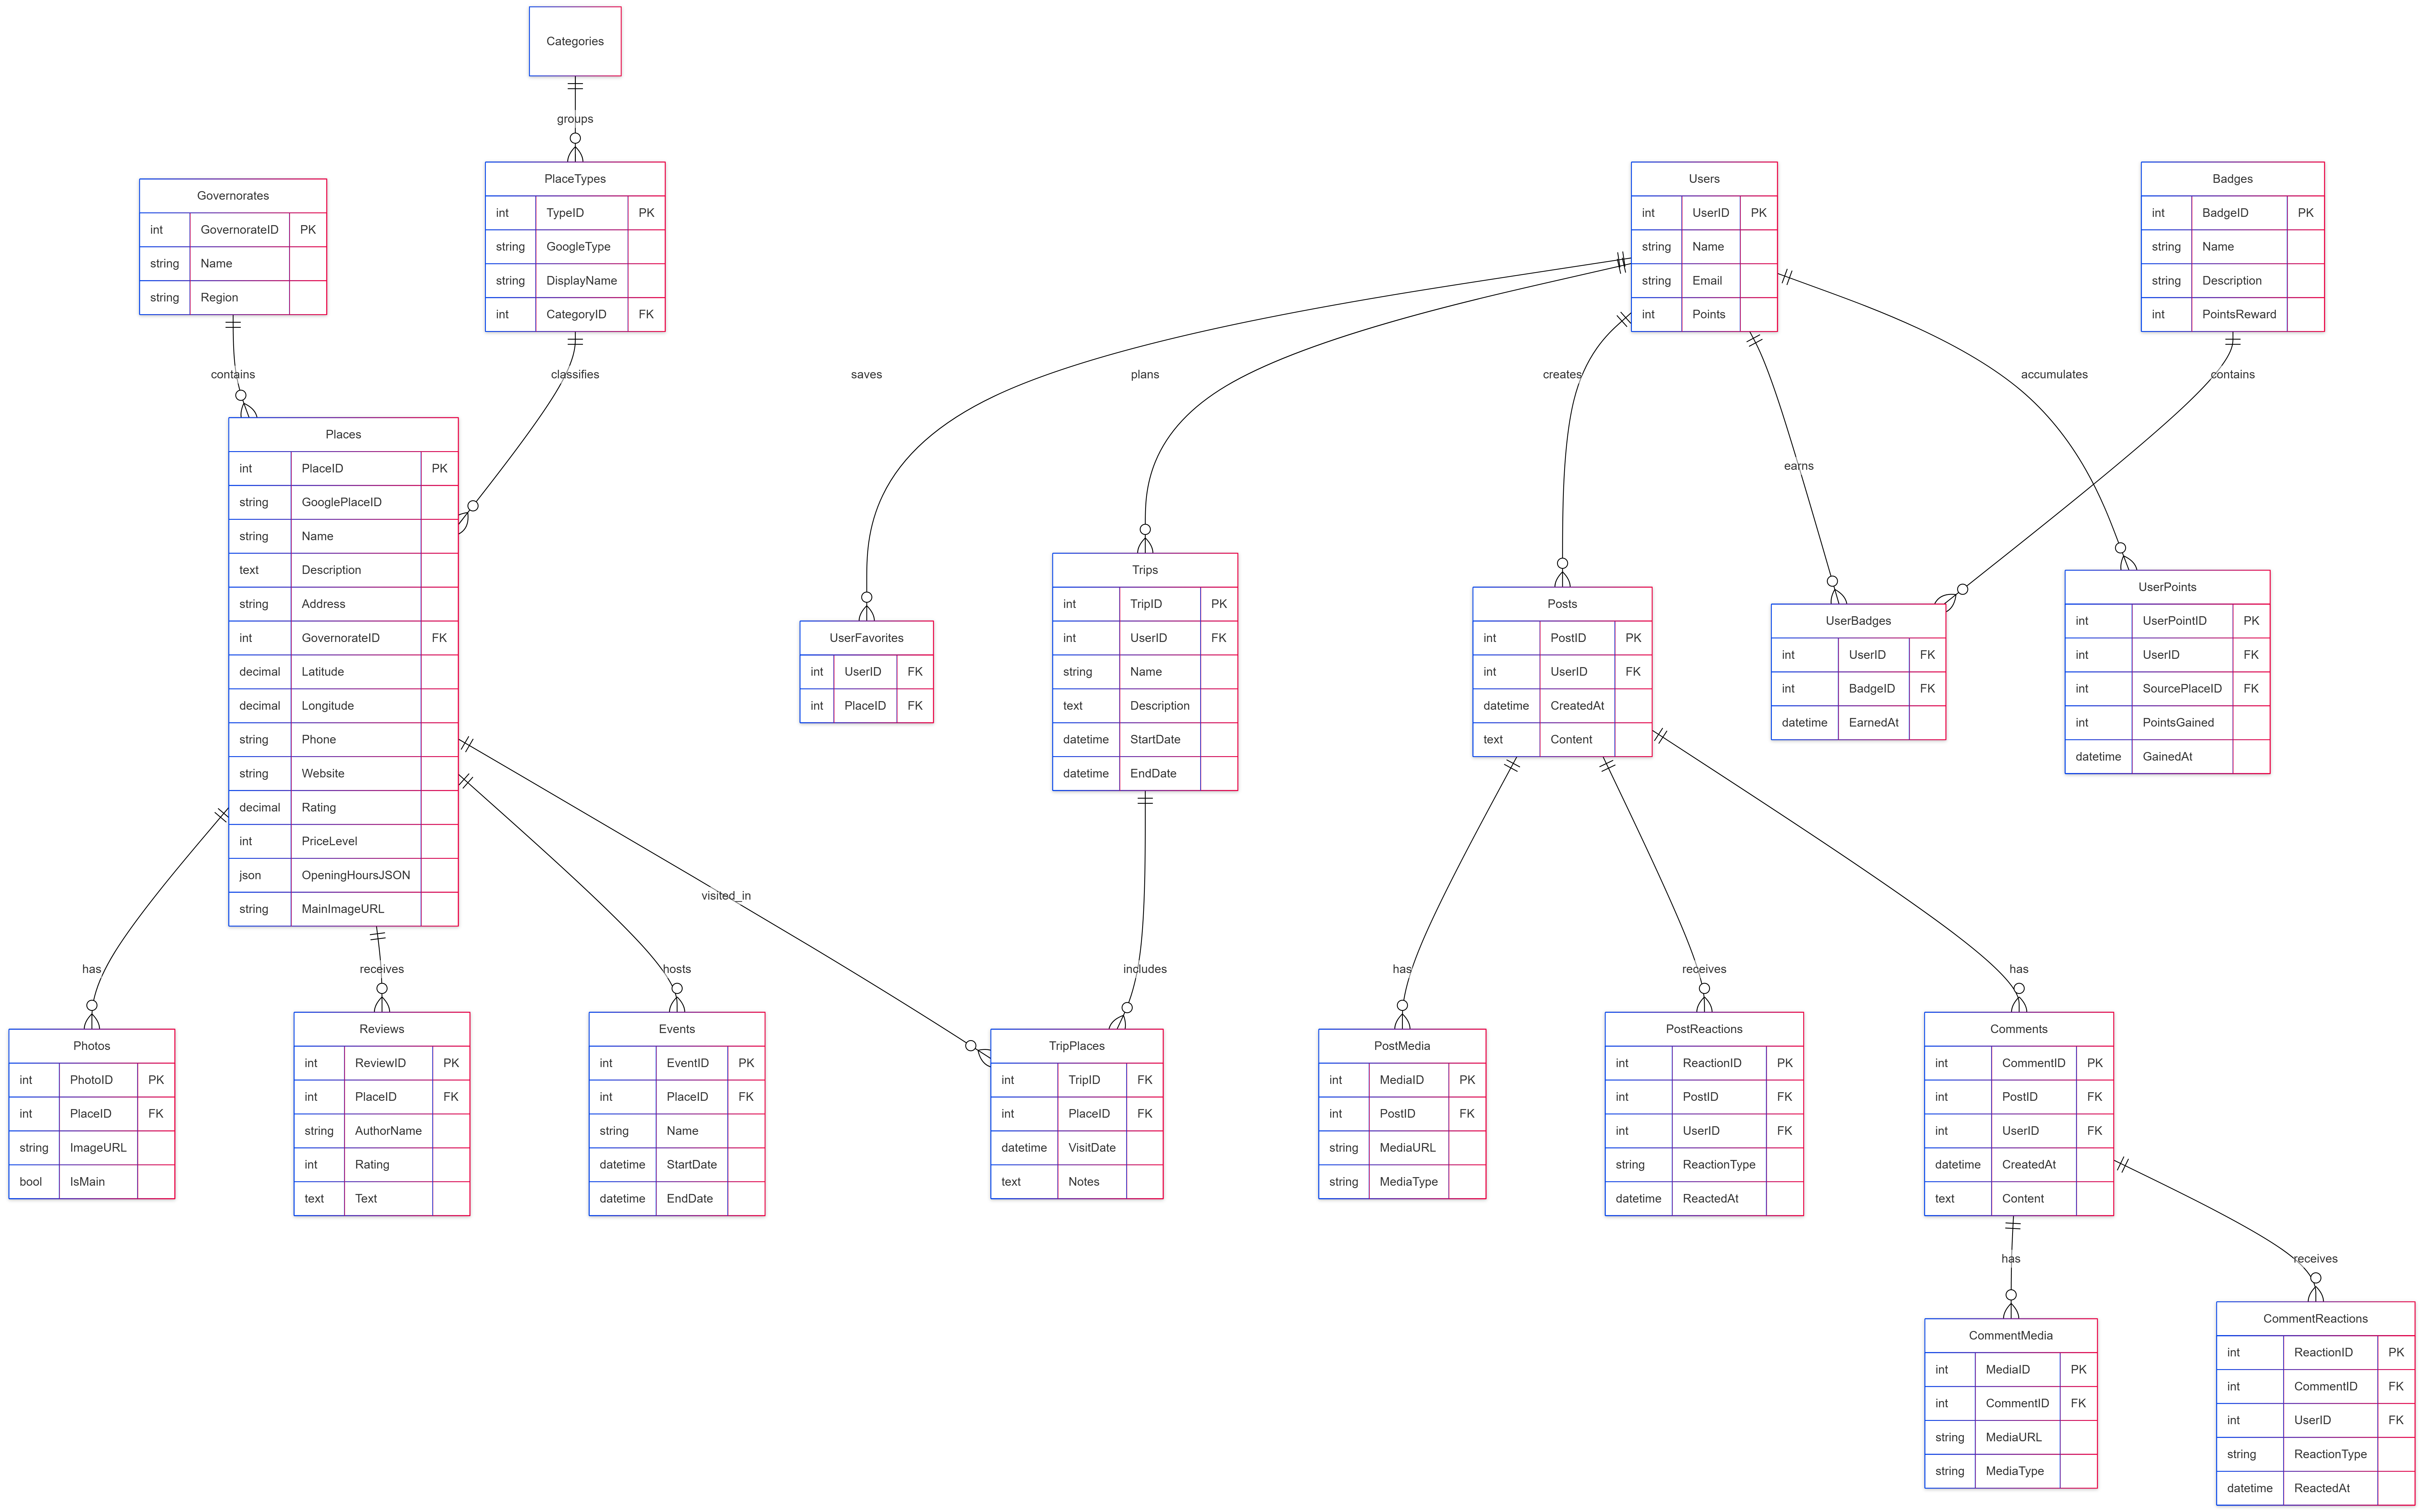
\includegraphics[width=0.9\textwidth]{figures/erd.png}
    \caption{Entity Relationship Diagram (ERD)}
    \label{fig:erd}

\end{figure}

\section{Frontend Architecture \& State Management Journey}
Building a visually rich, heavily interactive frontend for Kemora posed a significant challenge: State Management. Initially, passing state down the widget tree via constructors led to "prop drilling," making the UI rigid and difficult to test. 

To conquer this, we adopted the \textbf{Provider} pattern \cite{providerpattern}. Provider allowed us to cleanly separate our UI rendering from our business logic. By injecting ViewModels and Services at the top of the tree, any widget could reactively listen to state changes without tightly coupling to the data source. This decision transformed our Flutter application (\texttt{lib/presentation/}) into a highly modular, testable, and responsive frontend. The User Interface (UI) follows a "Modern Heritage" design language—blending contemporary mobile UX patterns (glassmorphism, vibrant gradients) with culturally resonant typography and color palettes.

Beyond state management, a robust \textbf{Mobile Security \& Offline Data Strategy} is implemented to ensure data integrity and user privacy. Sensitive credentials, such as JWTs and refresh tokens, are securely persisted using \textbf{Flutter Secure Storage}, leveraging native platform keystores. For performance and offline capabilities, frequently accessed data and user preferences are cached locally using high-performance embedded databases like \textbf{SQLite} and \textbf{Hive}, minimizing network overhead and allowing the application to gracefully handle intermittent connectivity.

\subsection{Journey 1: Onboarding \& Authentication}
The user is first greeted by an animated Splash Screen, followed by an educational Walkthrough. The Authentication flow supports standard registration and OAuth. It intercepts deep links for email confirmation and password resets.

\begin{figure}[H]
    \centering
    \begin{minipage}[t]{0.45\textwidth}
        \centering
        \vspace{0pt}
        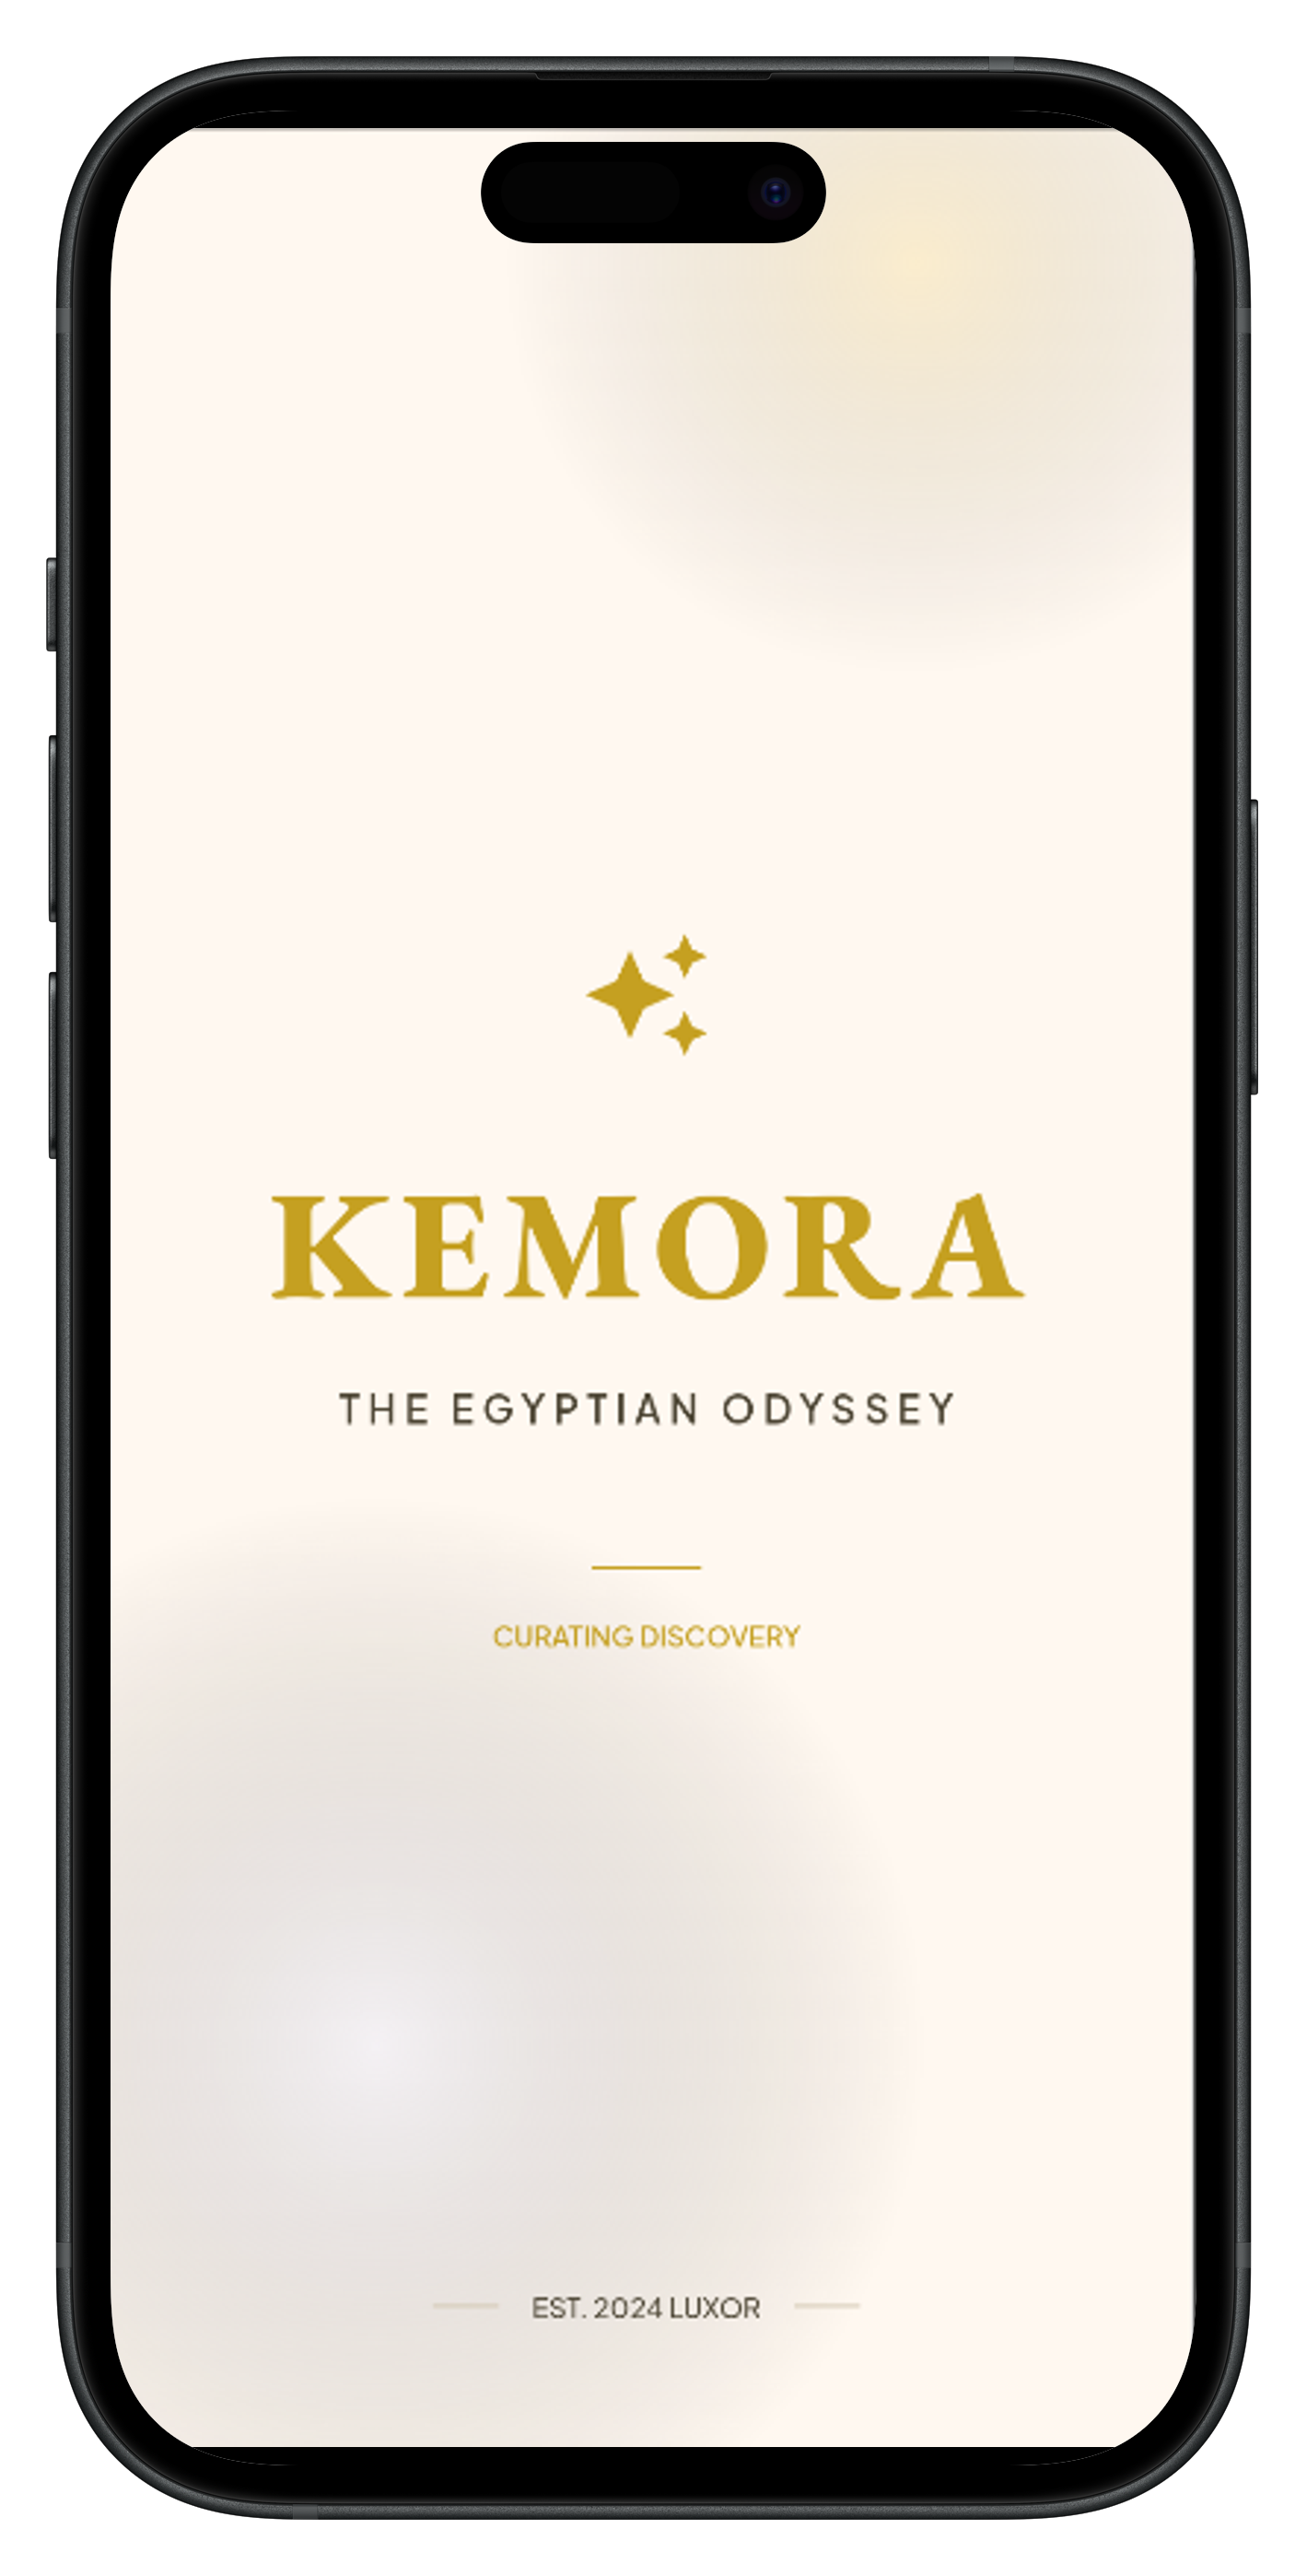
\includegraphics[width=\linewidth]{figures/splash.png}
        \caption{Mobile Application Splash Screen}
        \label{fig:splash}
    \end{minipage}\hfill
    \begin{minipage}[t]{0.45\textwidth}
        \centering
        \vspace{0pt}
        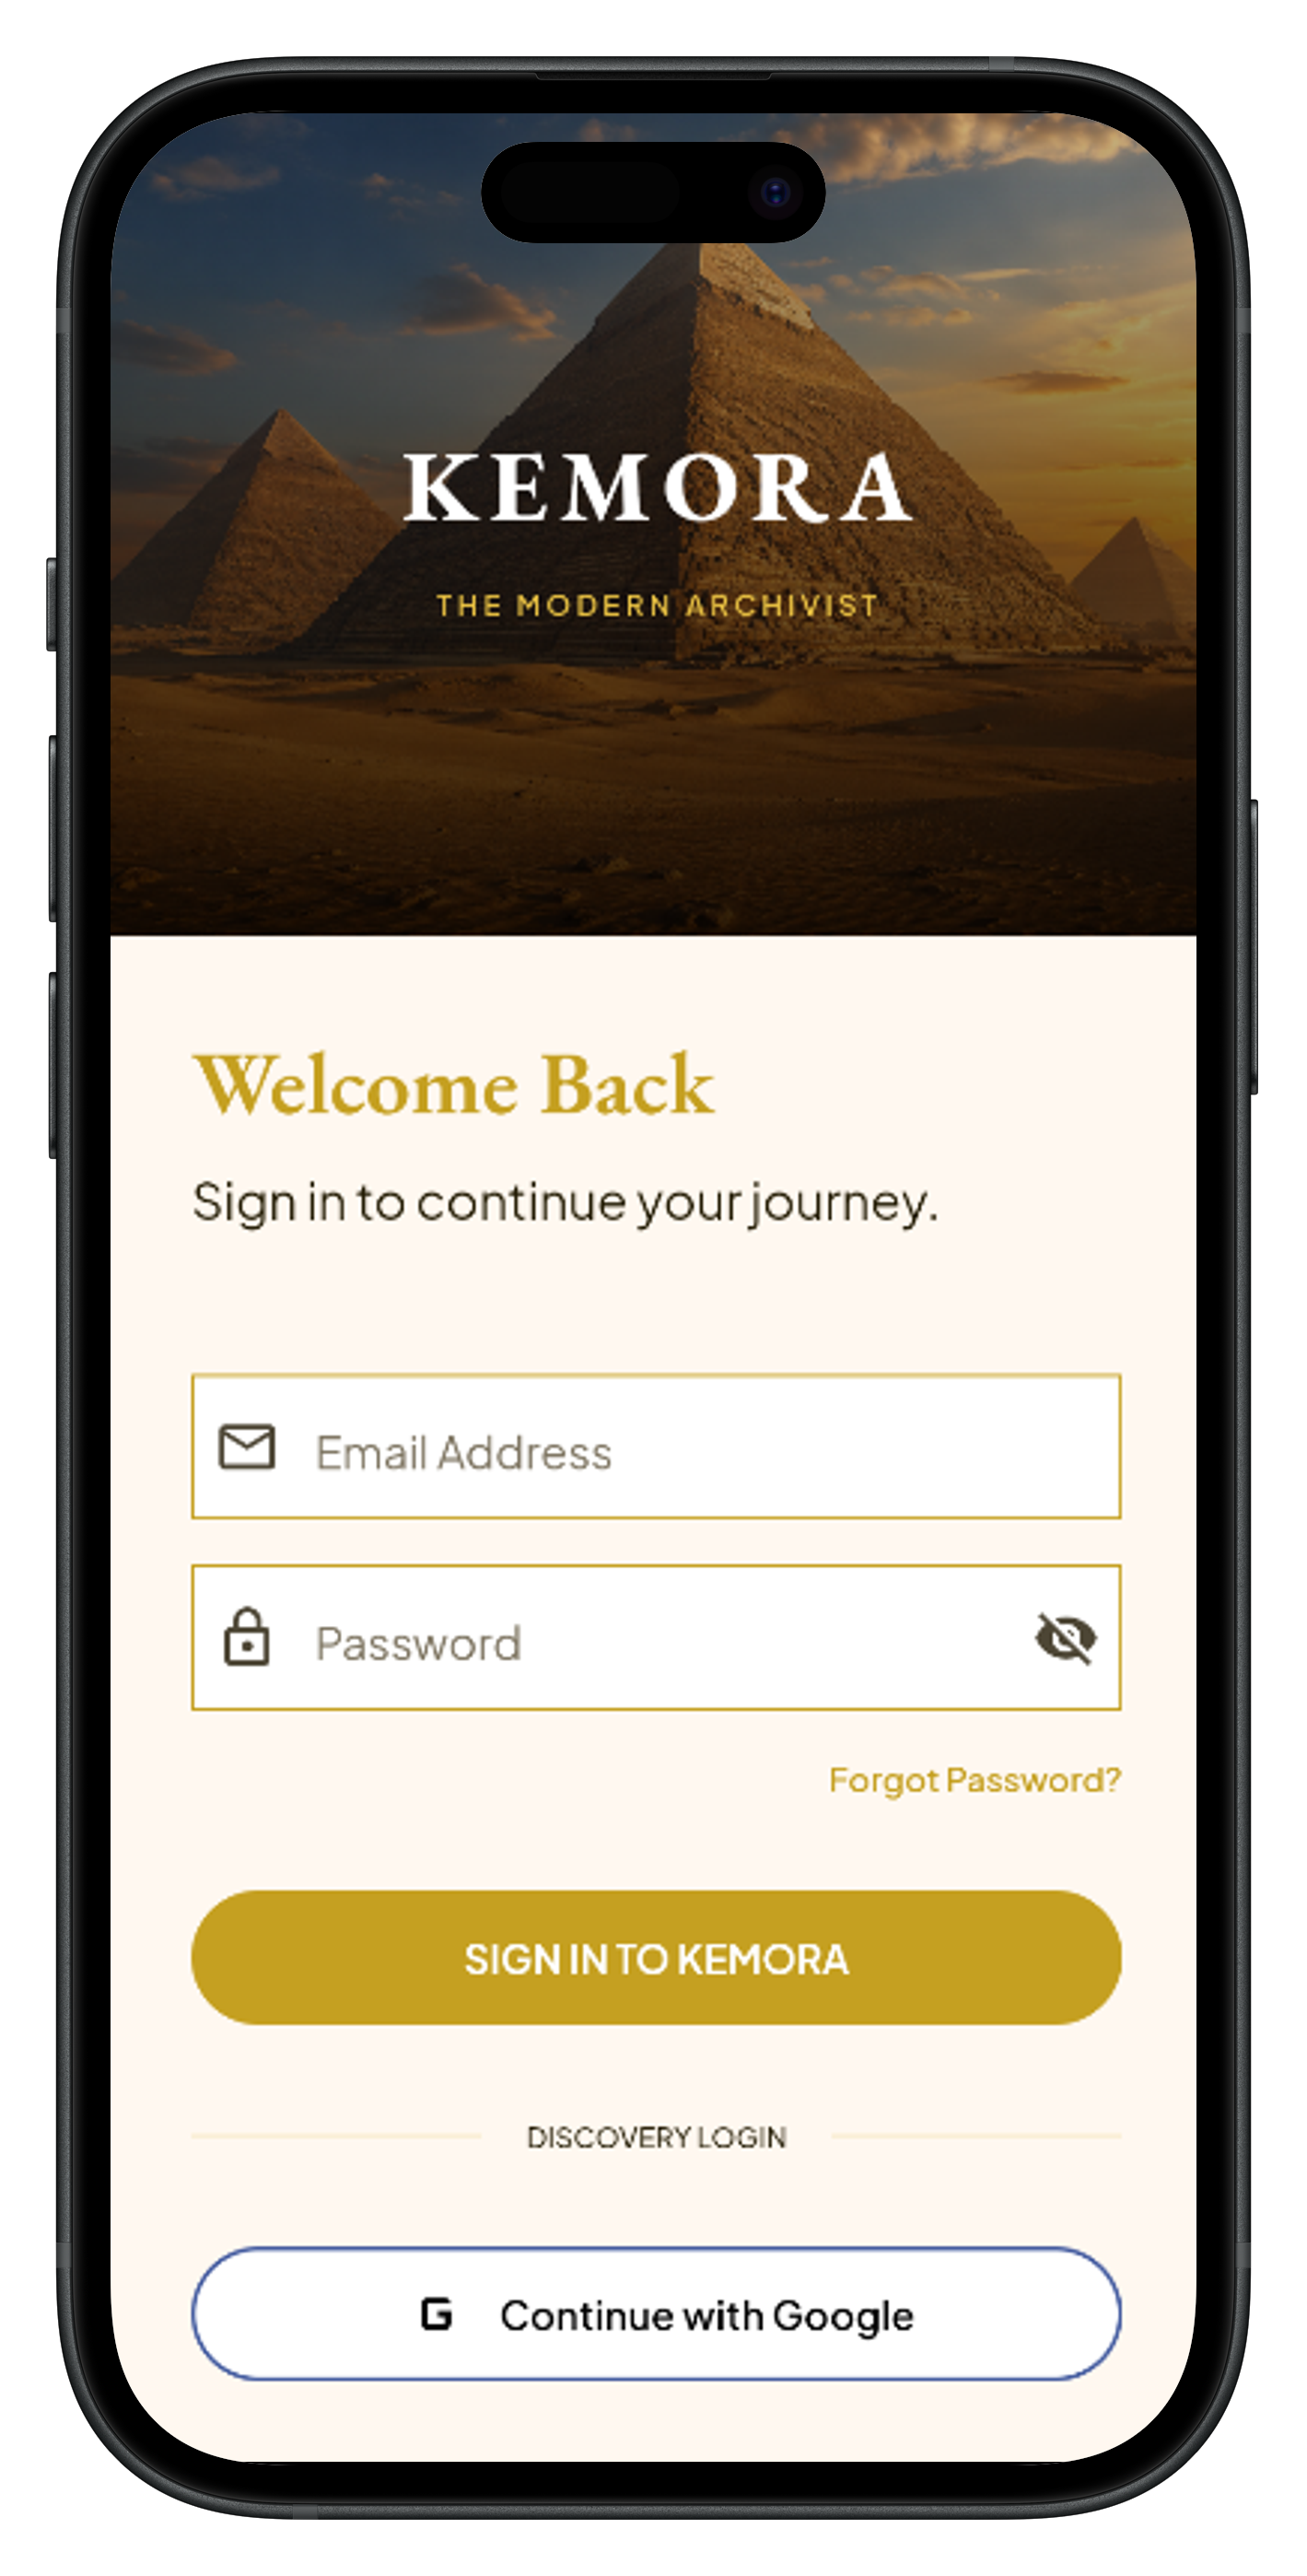
\includegraphics[width=\linewidth]{figures/login.png}
        \caption{Mobile Application Authentication Page}
        \label{fig:login}
    \end{minipage}
\end{figure}

\subsection{Journey 2: Main Dashboard \& Discovery}
The Home screen serves as the central hub, presenting personalized recommendations, top-rated destinations, and quick-action navigation via a custom floating tab bar.

\begin{figure}[H]
    \centering
    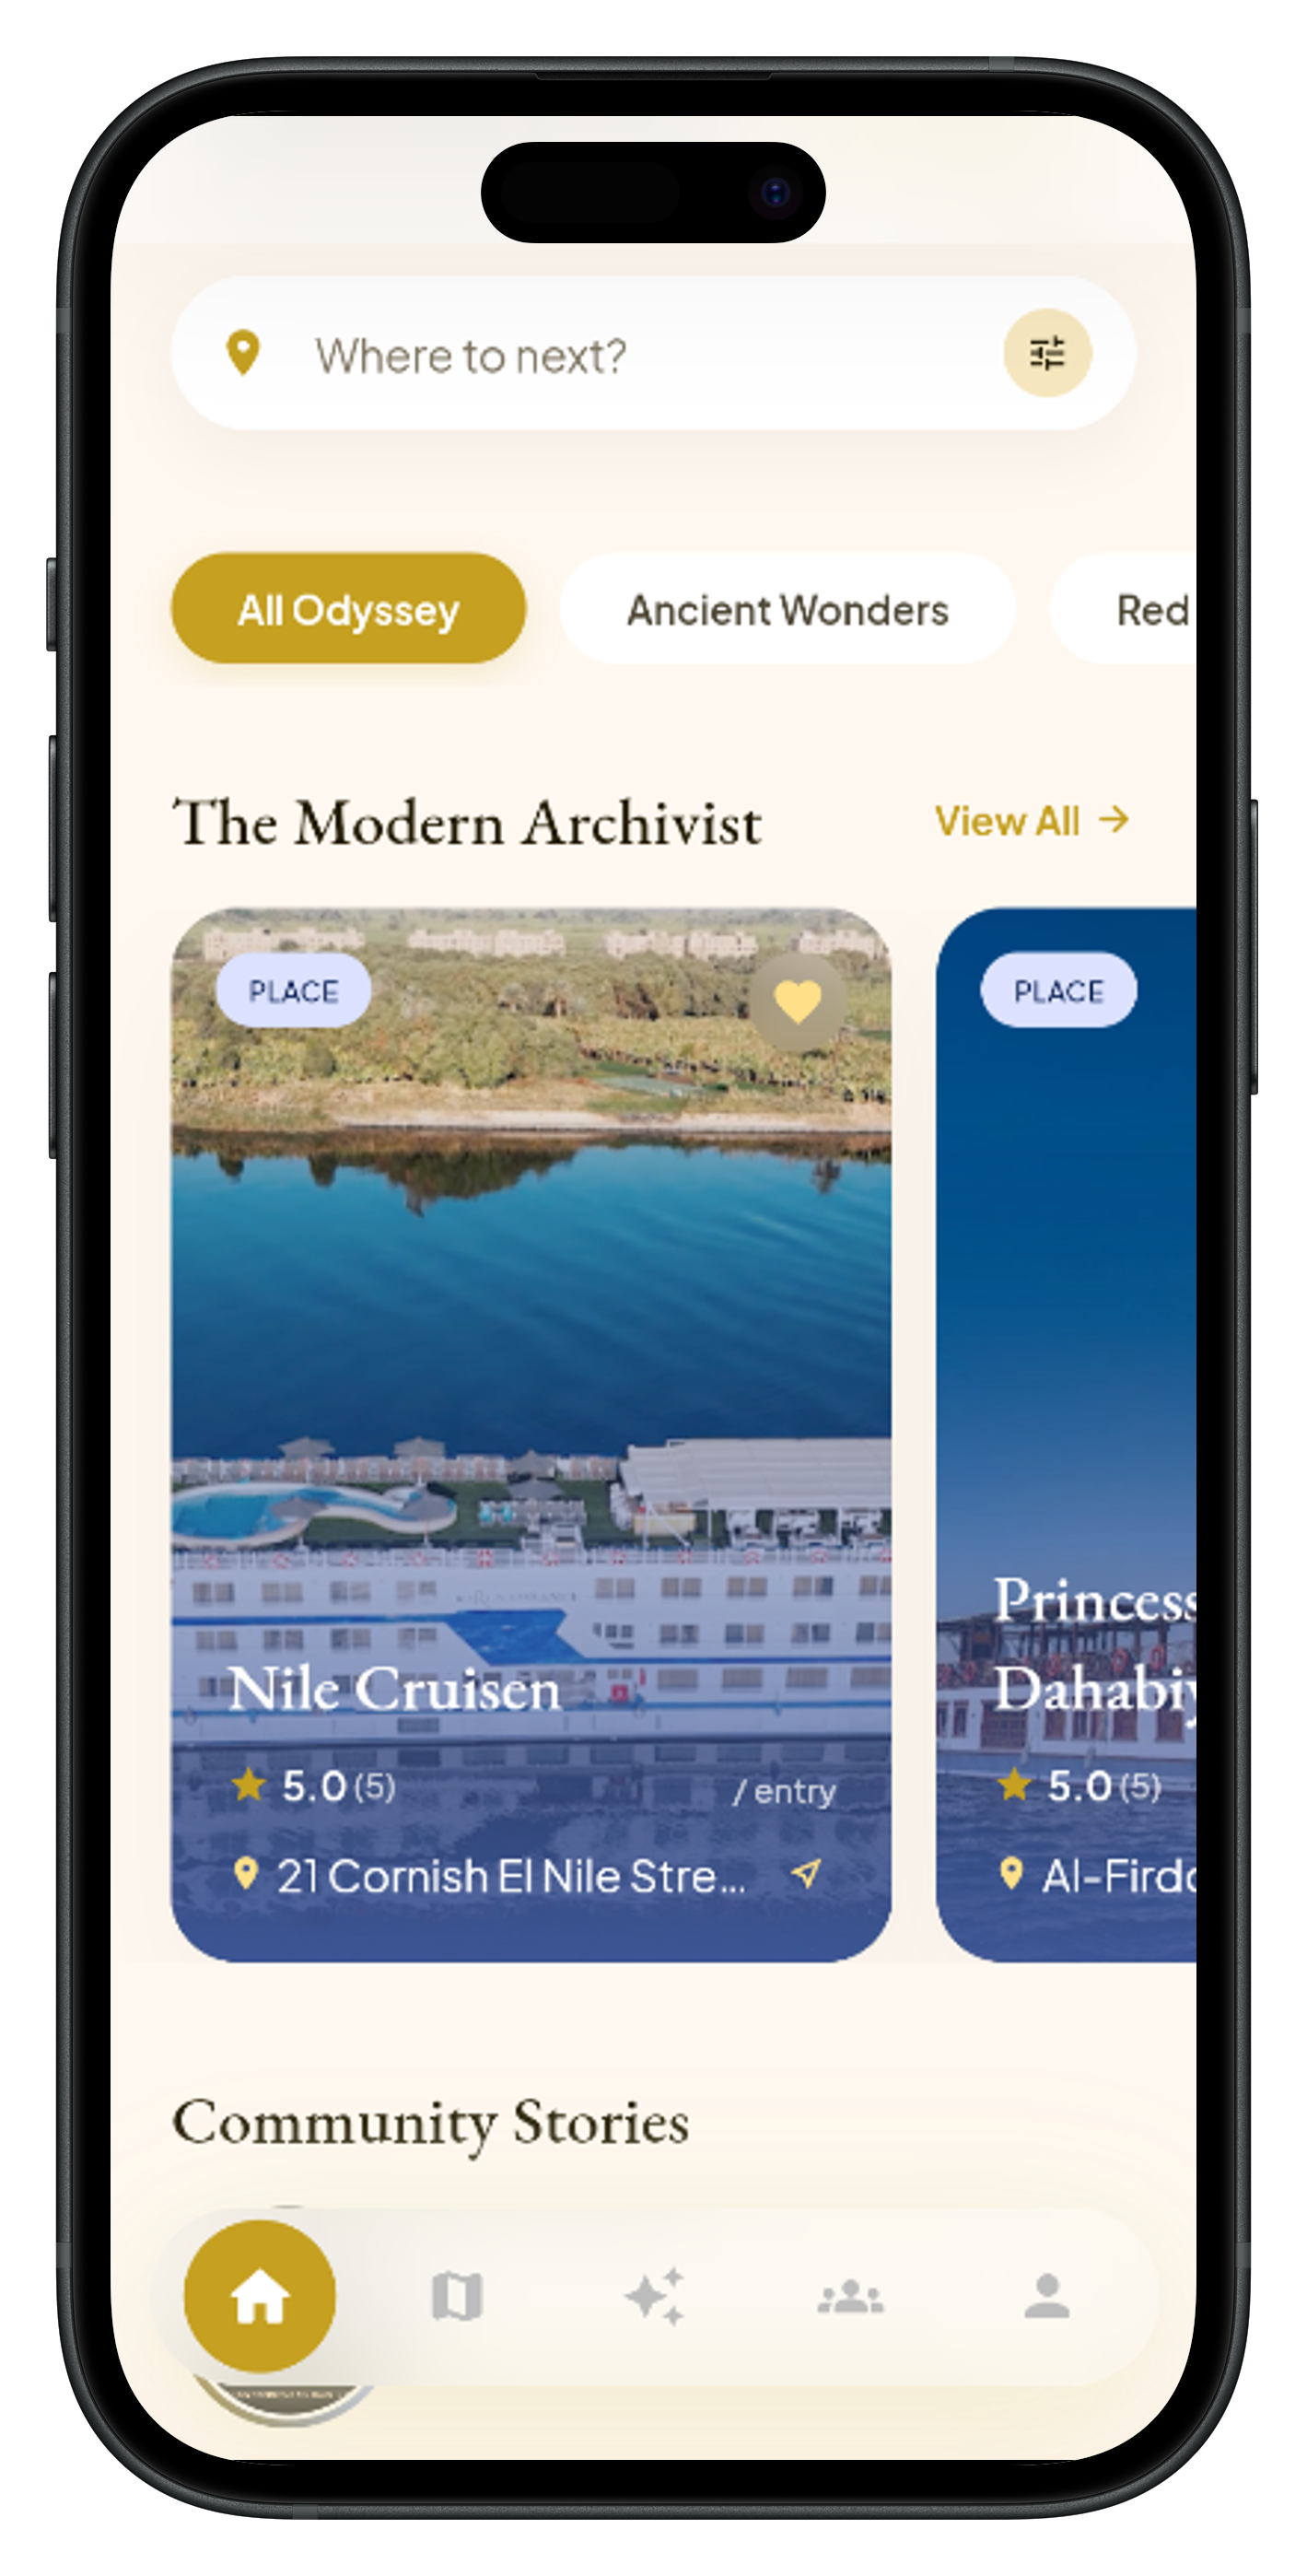
\includegraphics[width=0.45\textwidth]{figures/home.png}
    \caption{Mobile Application Home Page}
    \label{fig:home}
\end{figure}

\subsection{Journey 3: Explore \& Location Discovery}
Users can navigate an interactive map of Egyptian governorates. Selecting a governorate transitions to a detailed view listing sub-categories (Historical, Coastal, etc.) and individual Place detail screens.

\begin{figure}[H]
    \centering
    \begin{minipage}[t]{0.45\textwidth}
        \centering
        \vspace{0pt}
        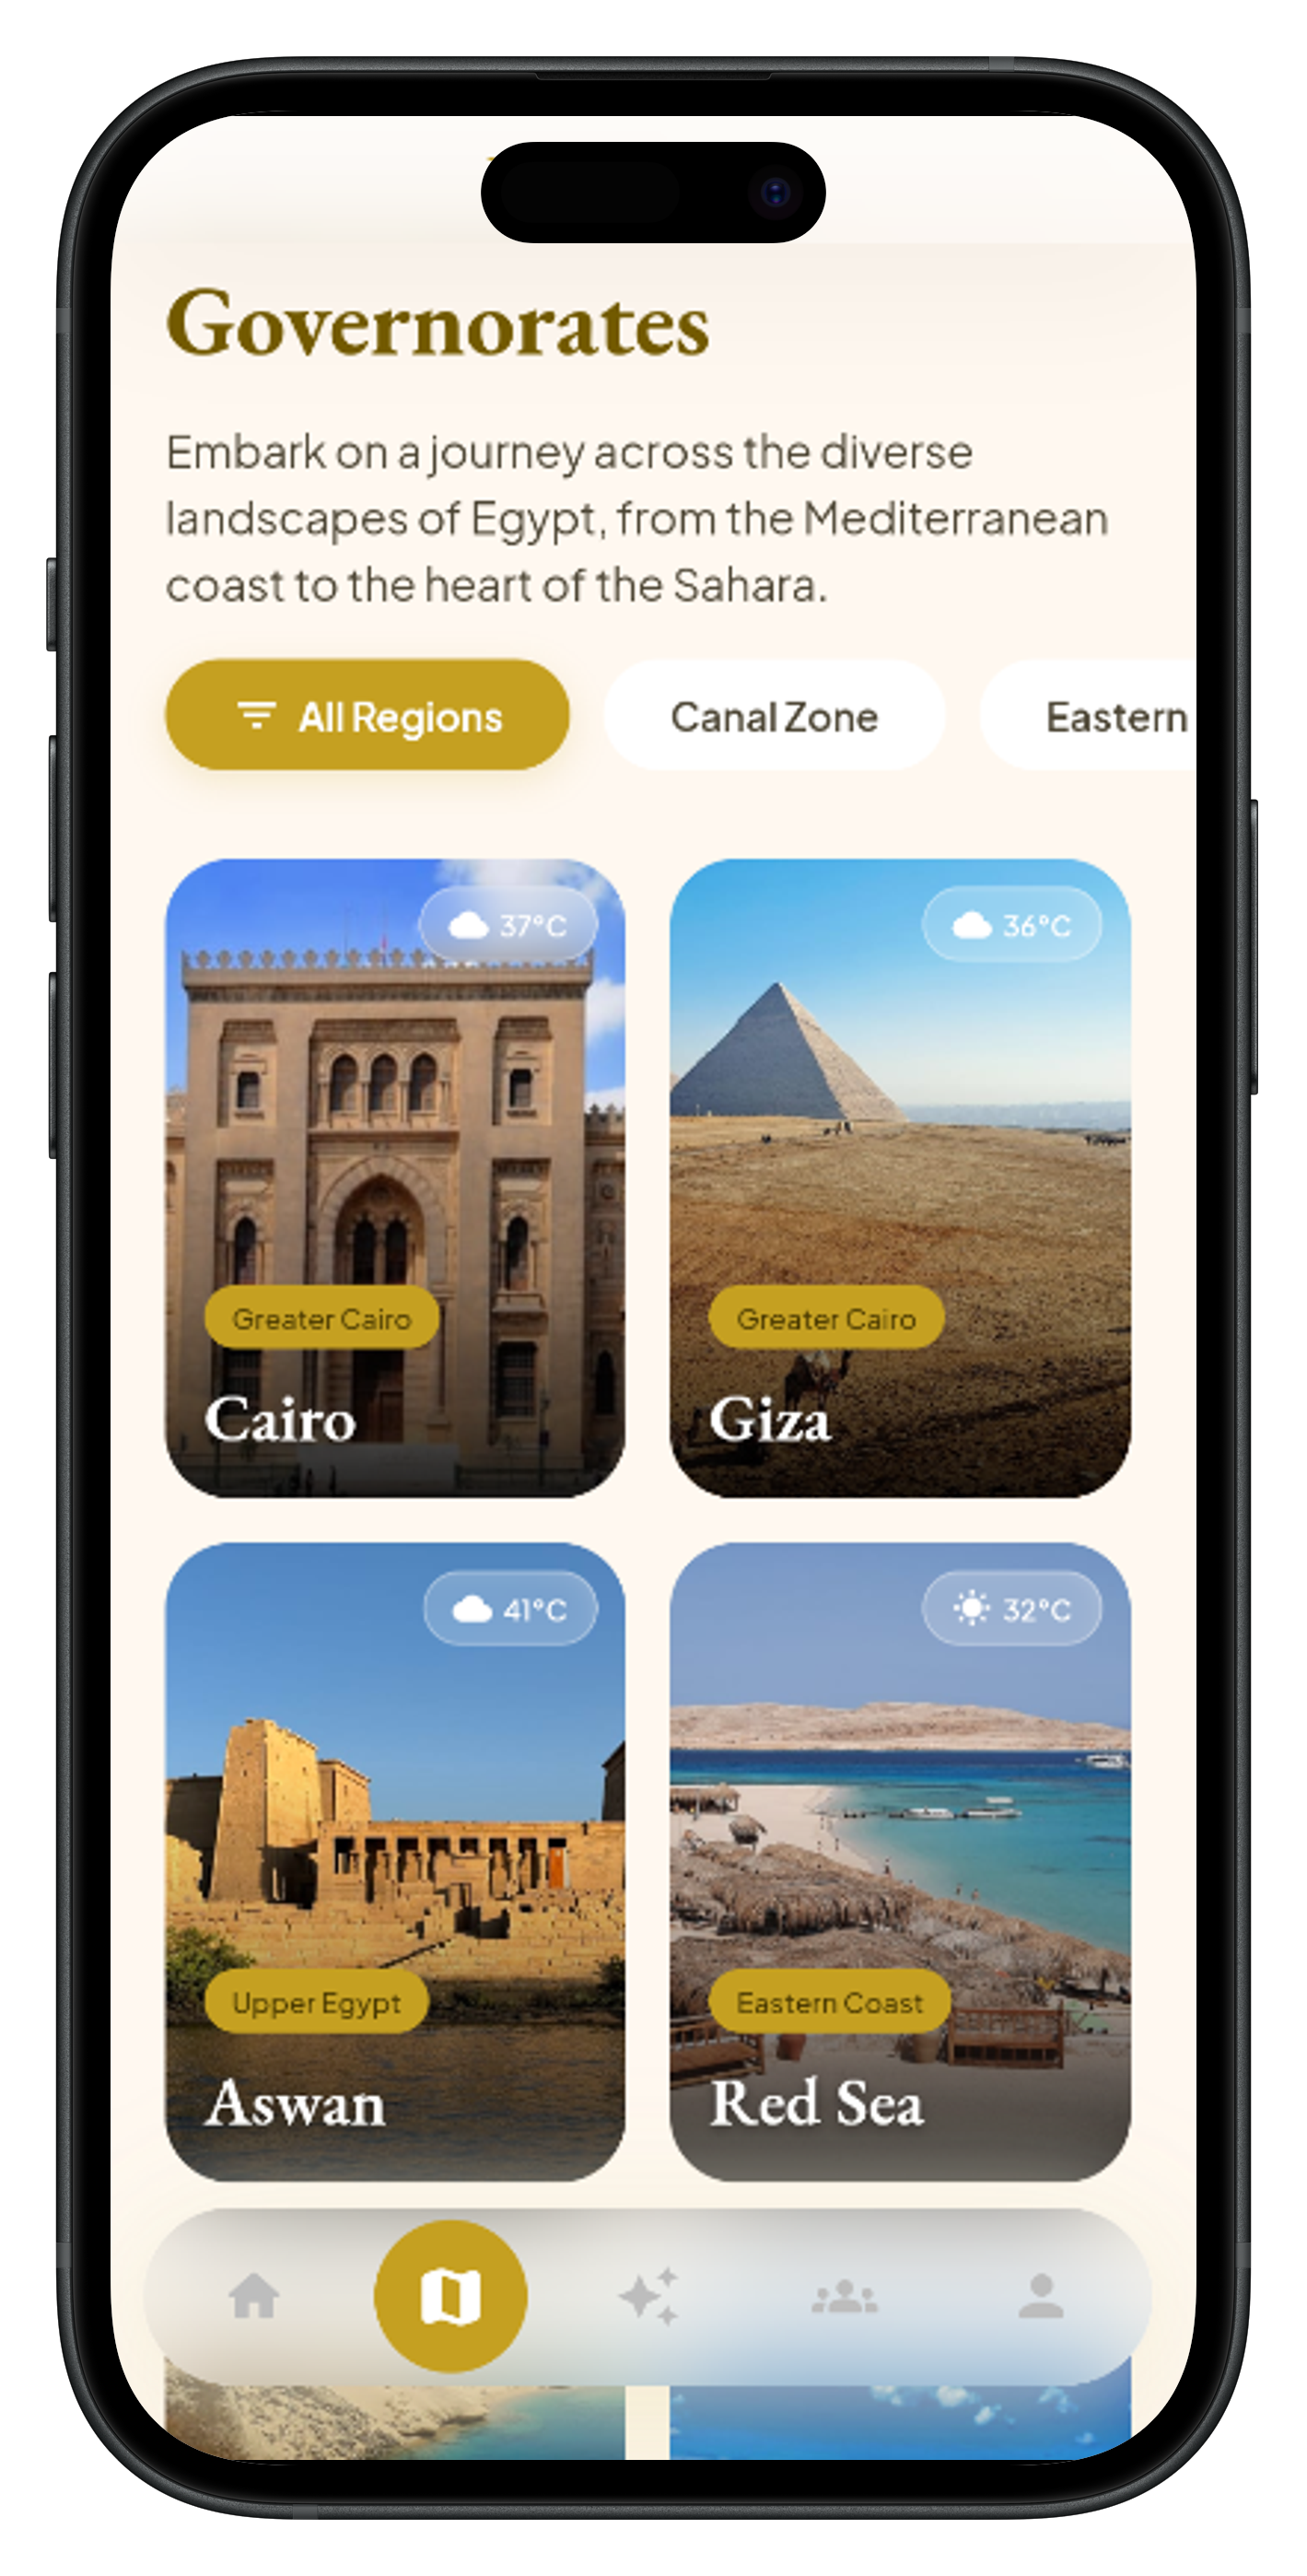
\includegraphics[width=\linewidth]{figures/gov_details.png}
        \caption{Governorate Details}
        \label{fig:gov_details}
    \end{minipage}\hfill
    \begin{minipage}[t]{0.45\textwidth}
        \centering
        \vspace{0pt}
        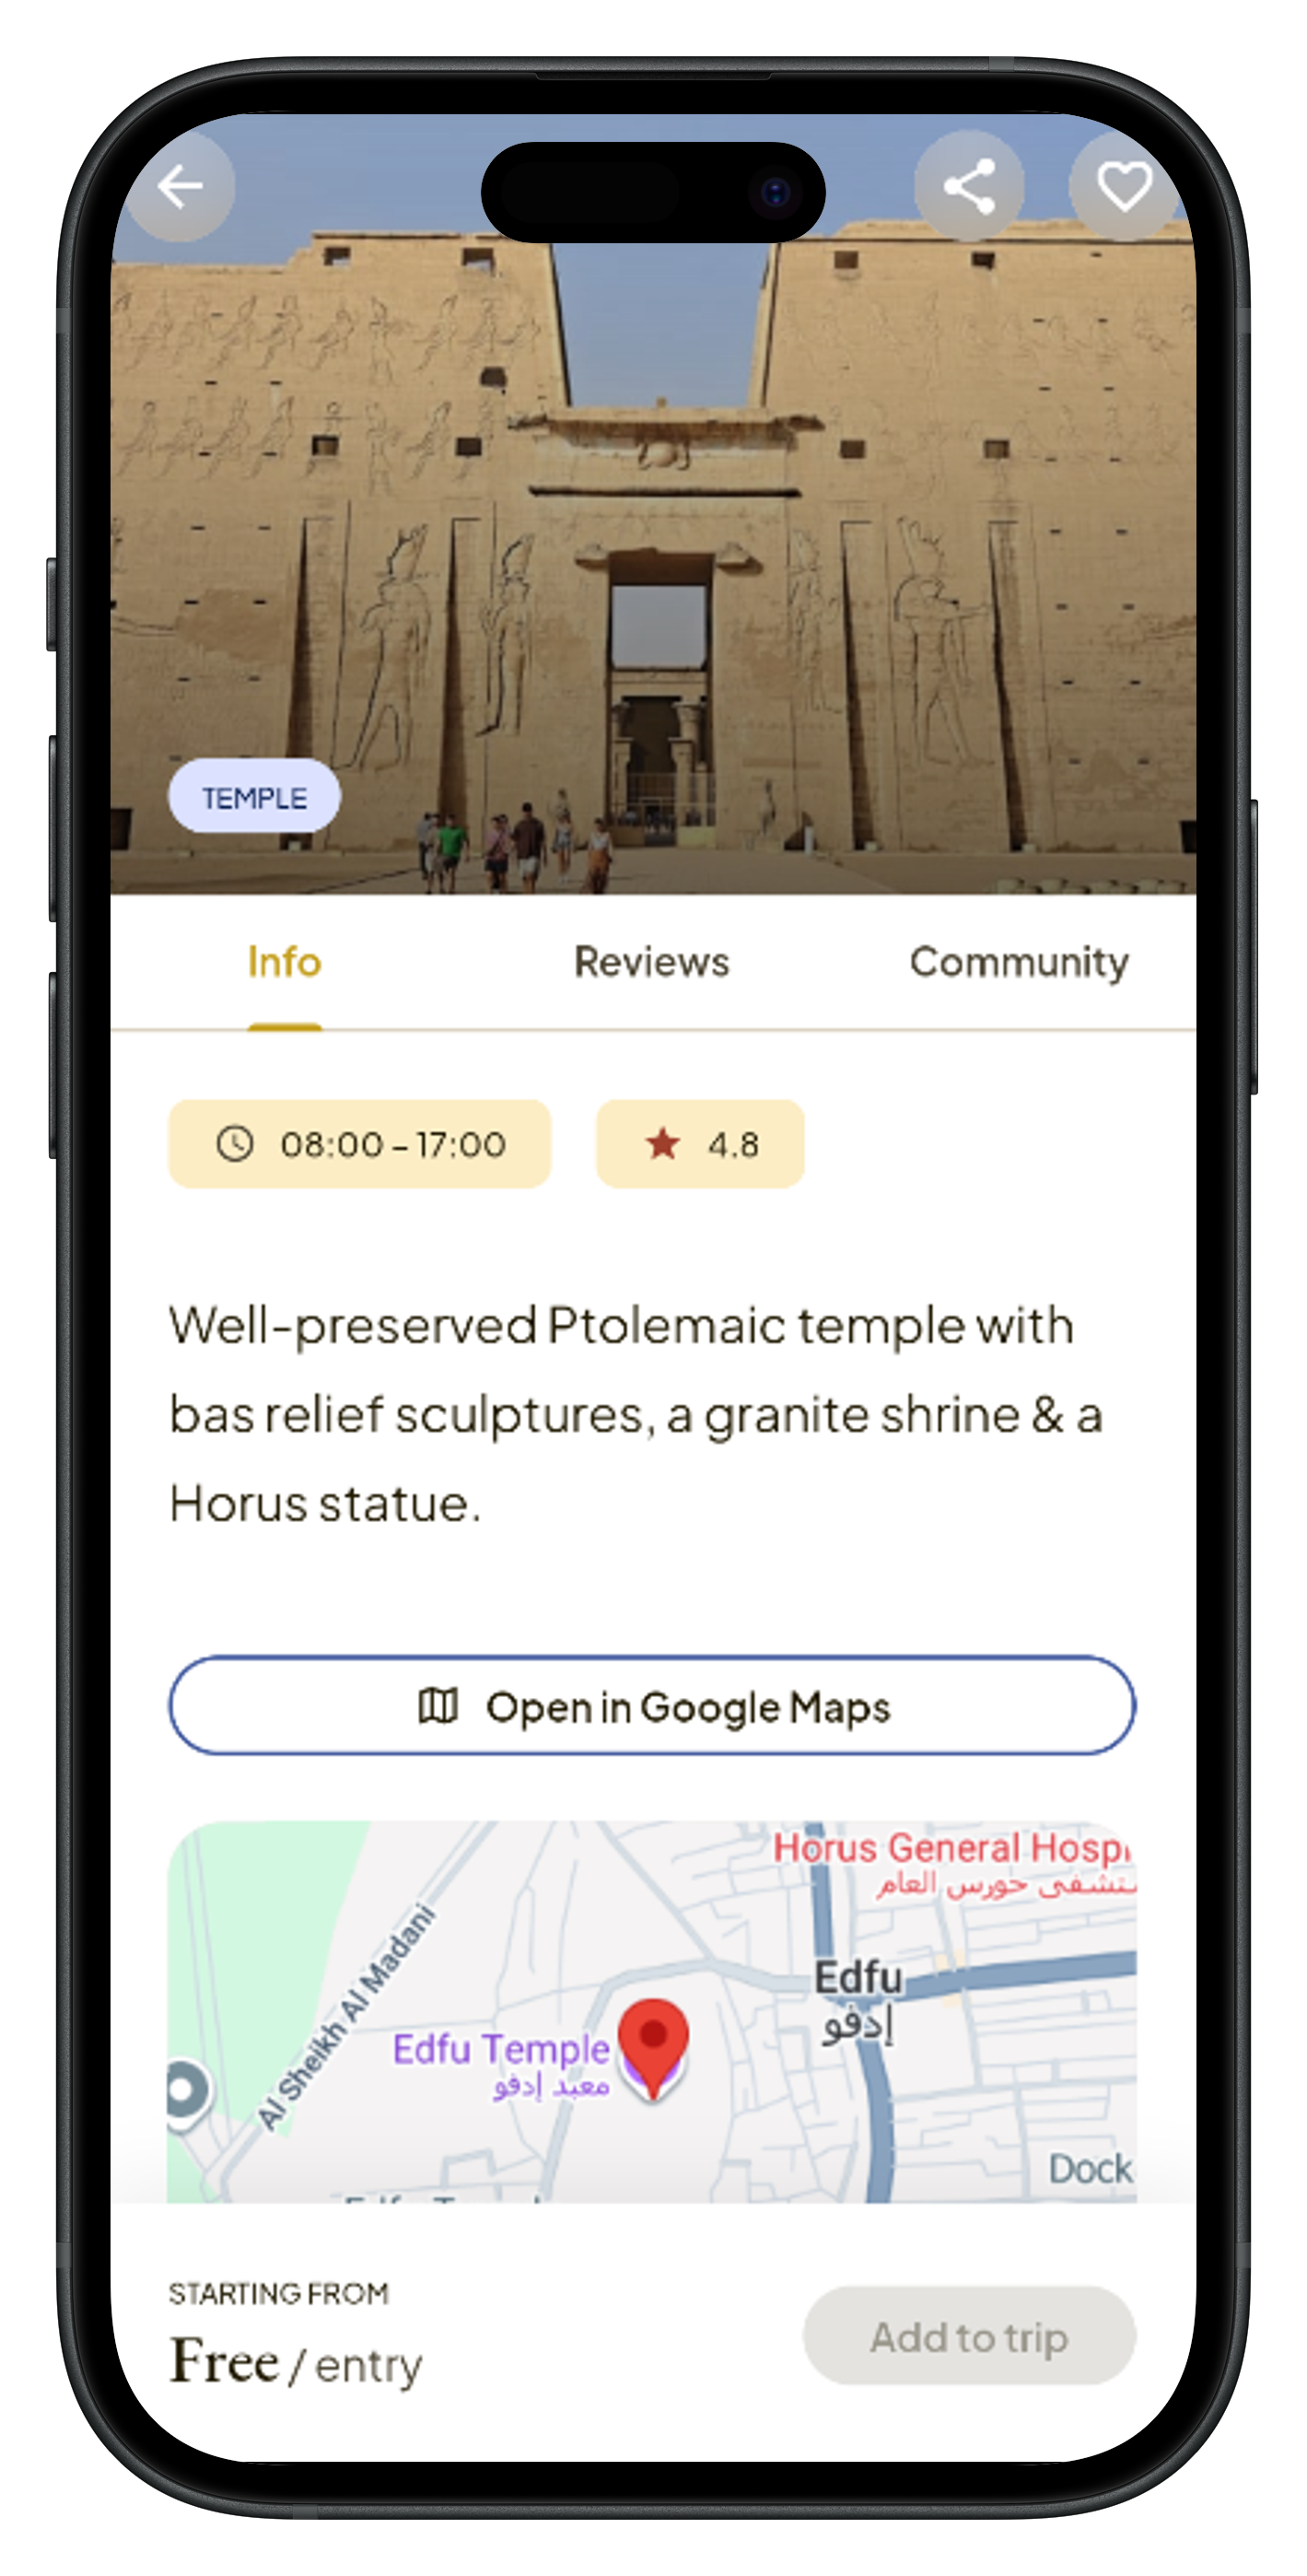
\includegraphics[width=\linewidth]{figures/place_details.png}
        \caption{Place Details}
        \label{fig:place_details}
    \end{minipage}
\end{figure}

\subsection{Journey 4: Trip Planning \& AI Itinerary}
This is the flagship journey. Users input parameters into a multi-step questionnaire (\texttt{ai\_step\_questions\_screen.dart}). The system displays a loading animation while negotiating with the backend AI. The result is a beautifully rendered, interactive timeline (\texttt{ai\_itinerary\_result\_screen.dart}).

\begin{figure}[H]
    \centering
    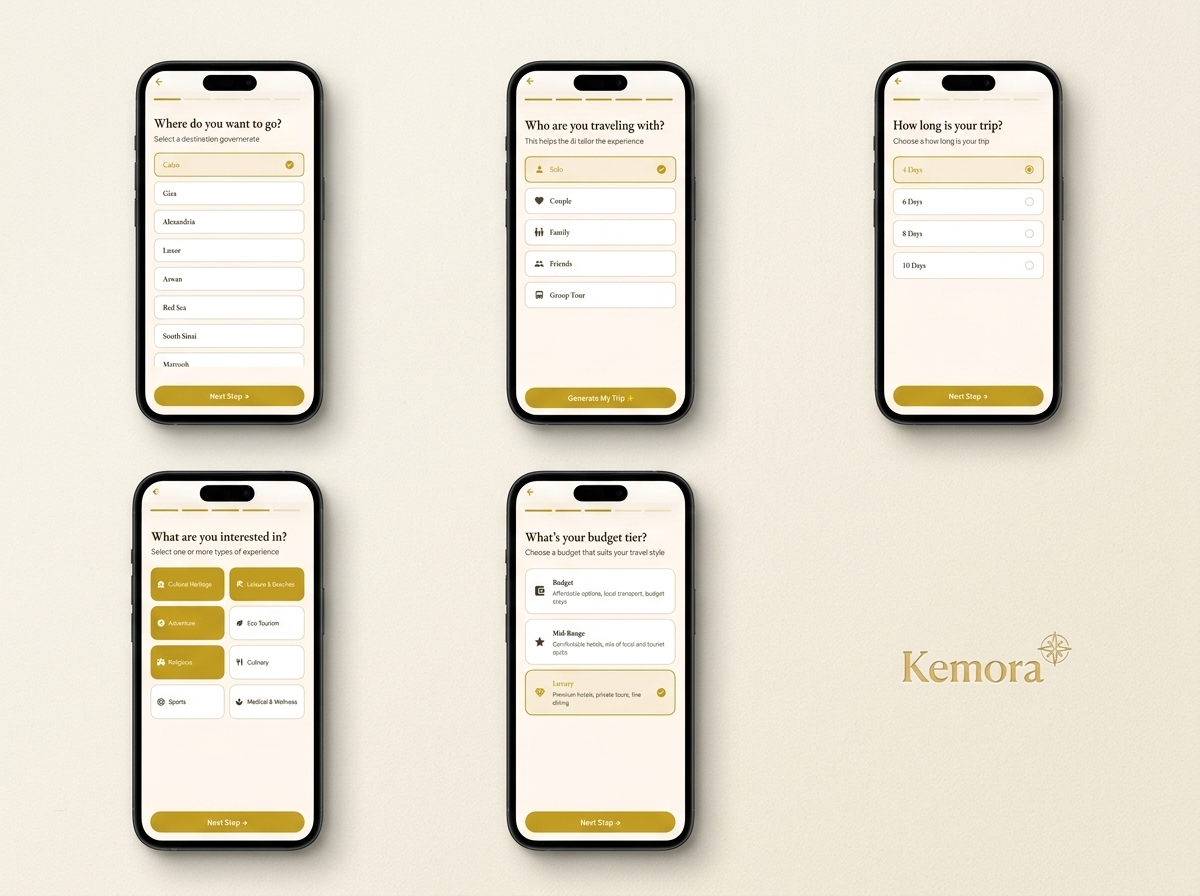
\includegraphics[width=\textwidth]{figures/ai_questions.png}
    \caption{AI Trip Planner Questionnaire}
    \label{fig:ai_questions}
\end{figure}

\subsection{Journey 5: Social \& Community}
A familiar, vertically scrolling feed allows users to consume and produce content. Users can view detailed posts and engage in comment threads.

\begin{figure}[H]
    \centering
    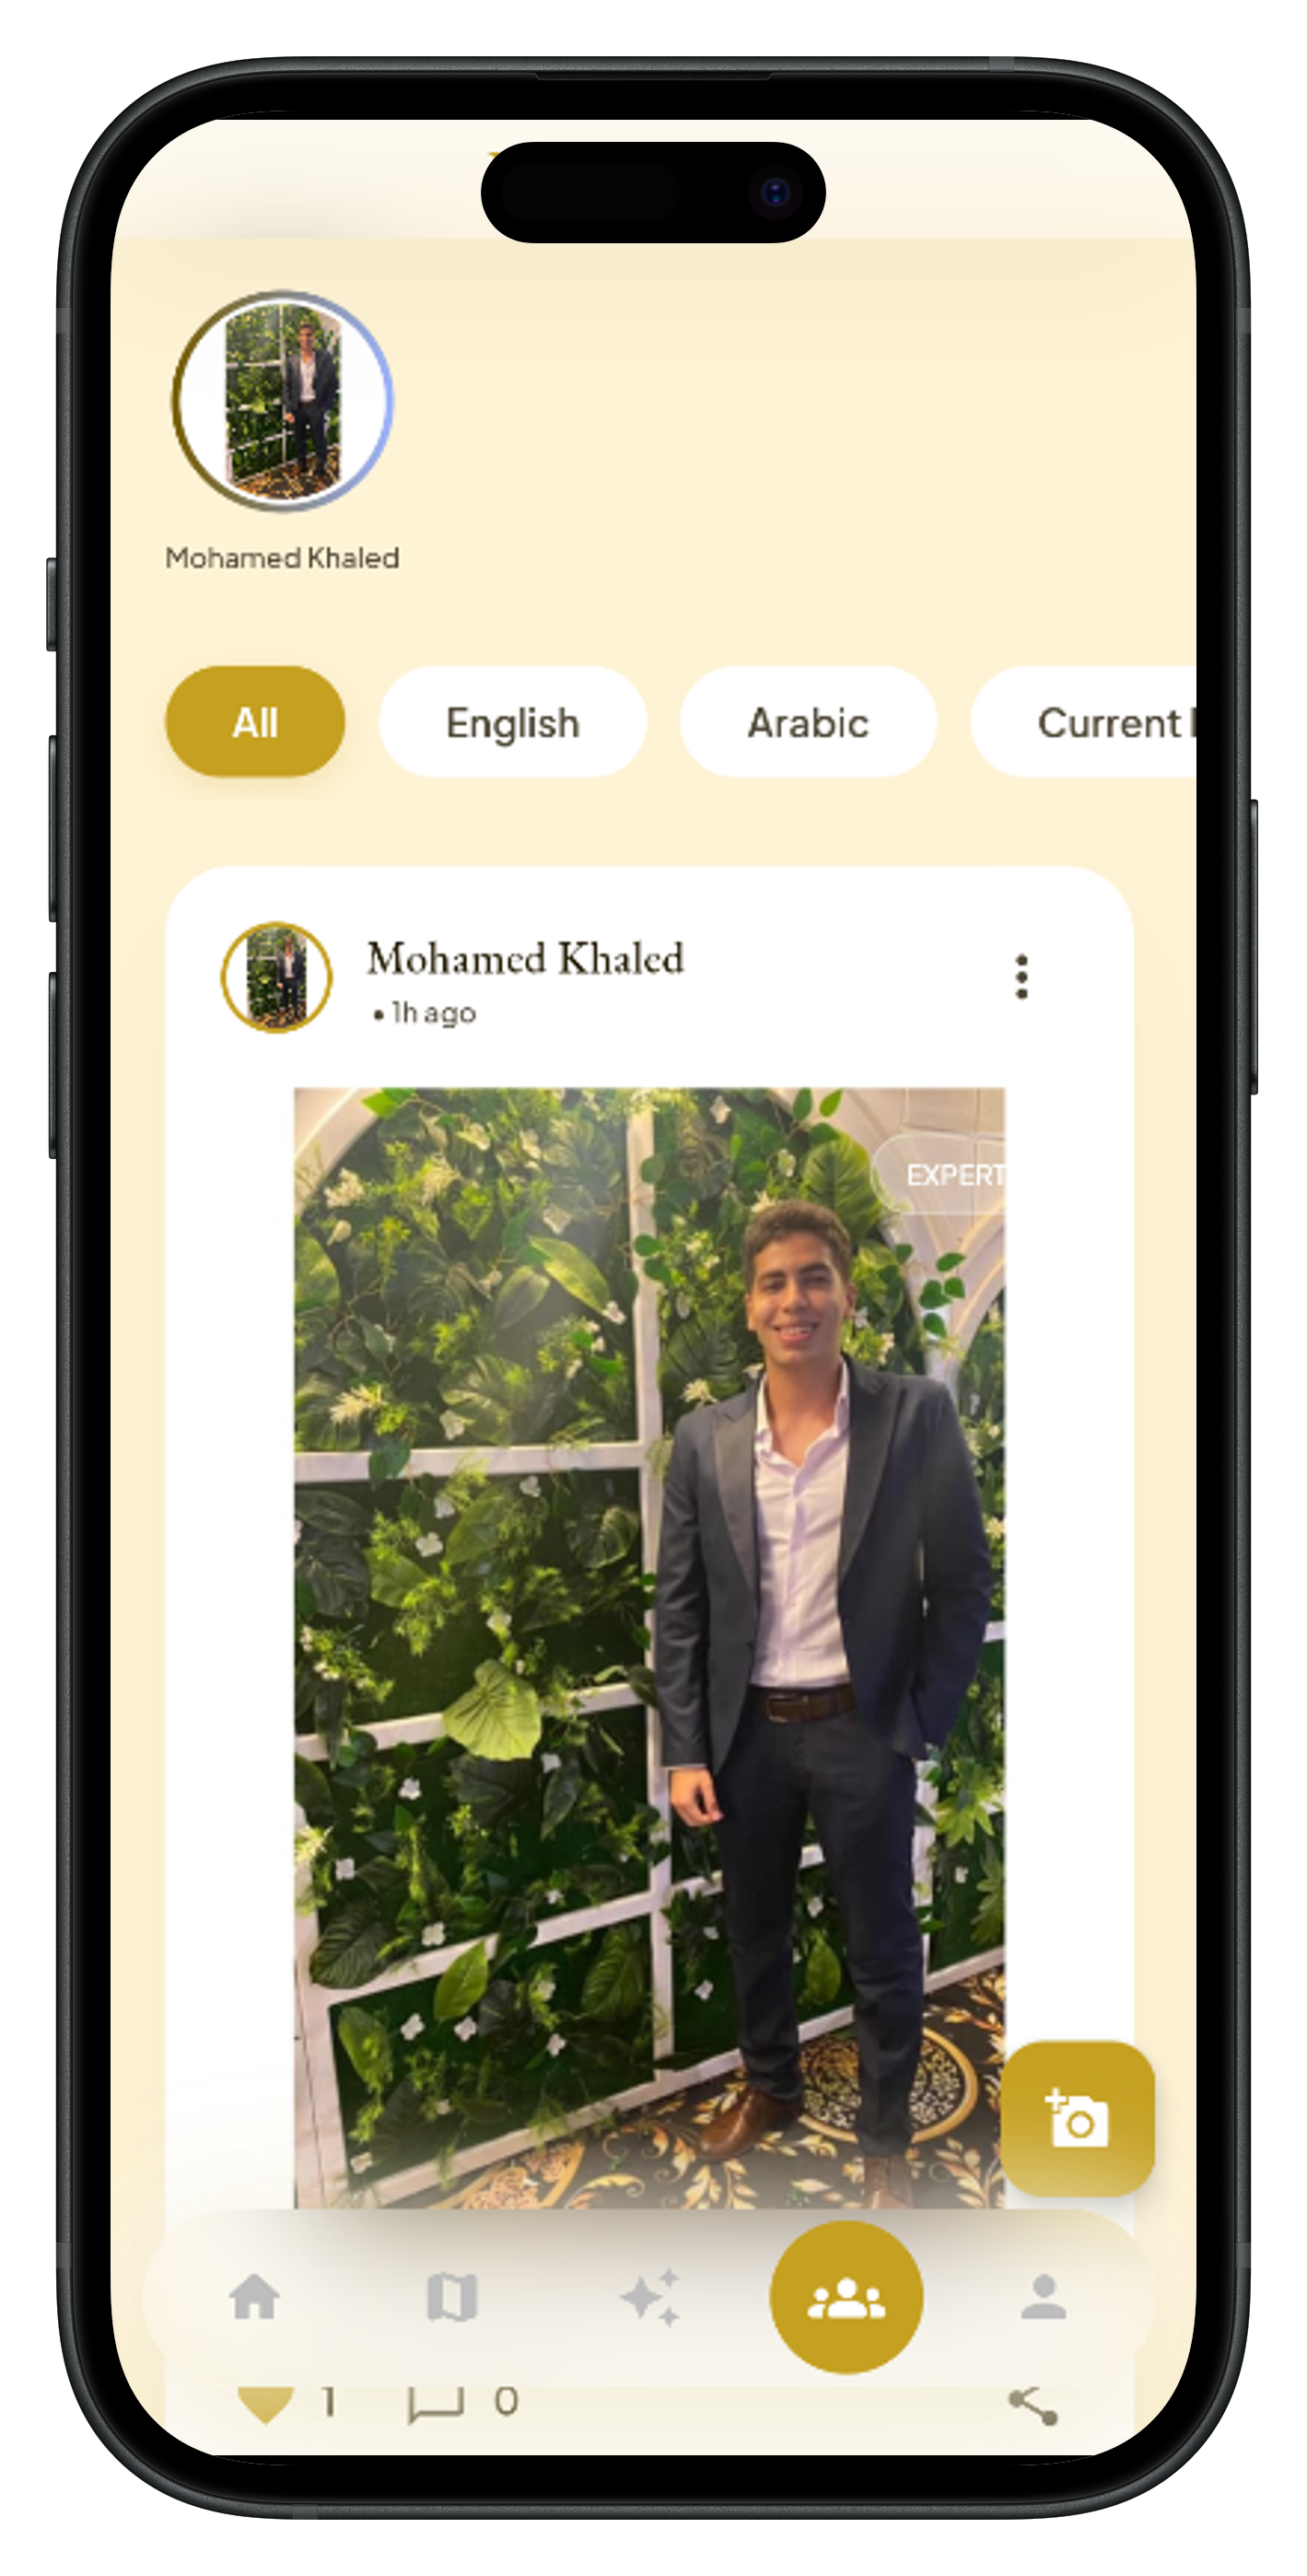
\includegraphics[width=0.45\textwidth]{figures/social_feed.png}
    \caption{Community Social Feed}
    \label{fig:social_feed}
\end{figure}

\subsection{Journey 6: Profile \& Gamification}
The Profile screen tracks the user's identity, displaying earned badges, total points, redeemed vouchers, and saved places.

\begin{figure}[H]
    \centering
    \begin{minipage}[t]{0.45\textwidth}
        \centering
        \vspace{0pt}
        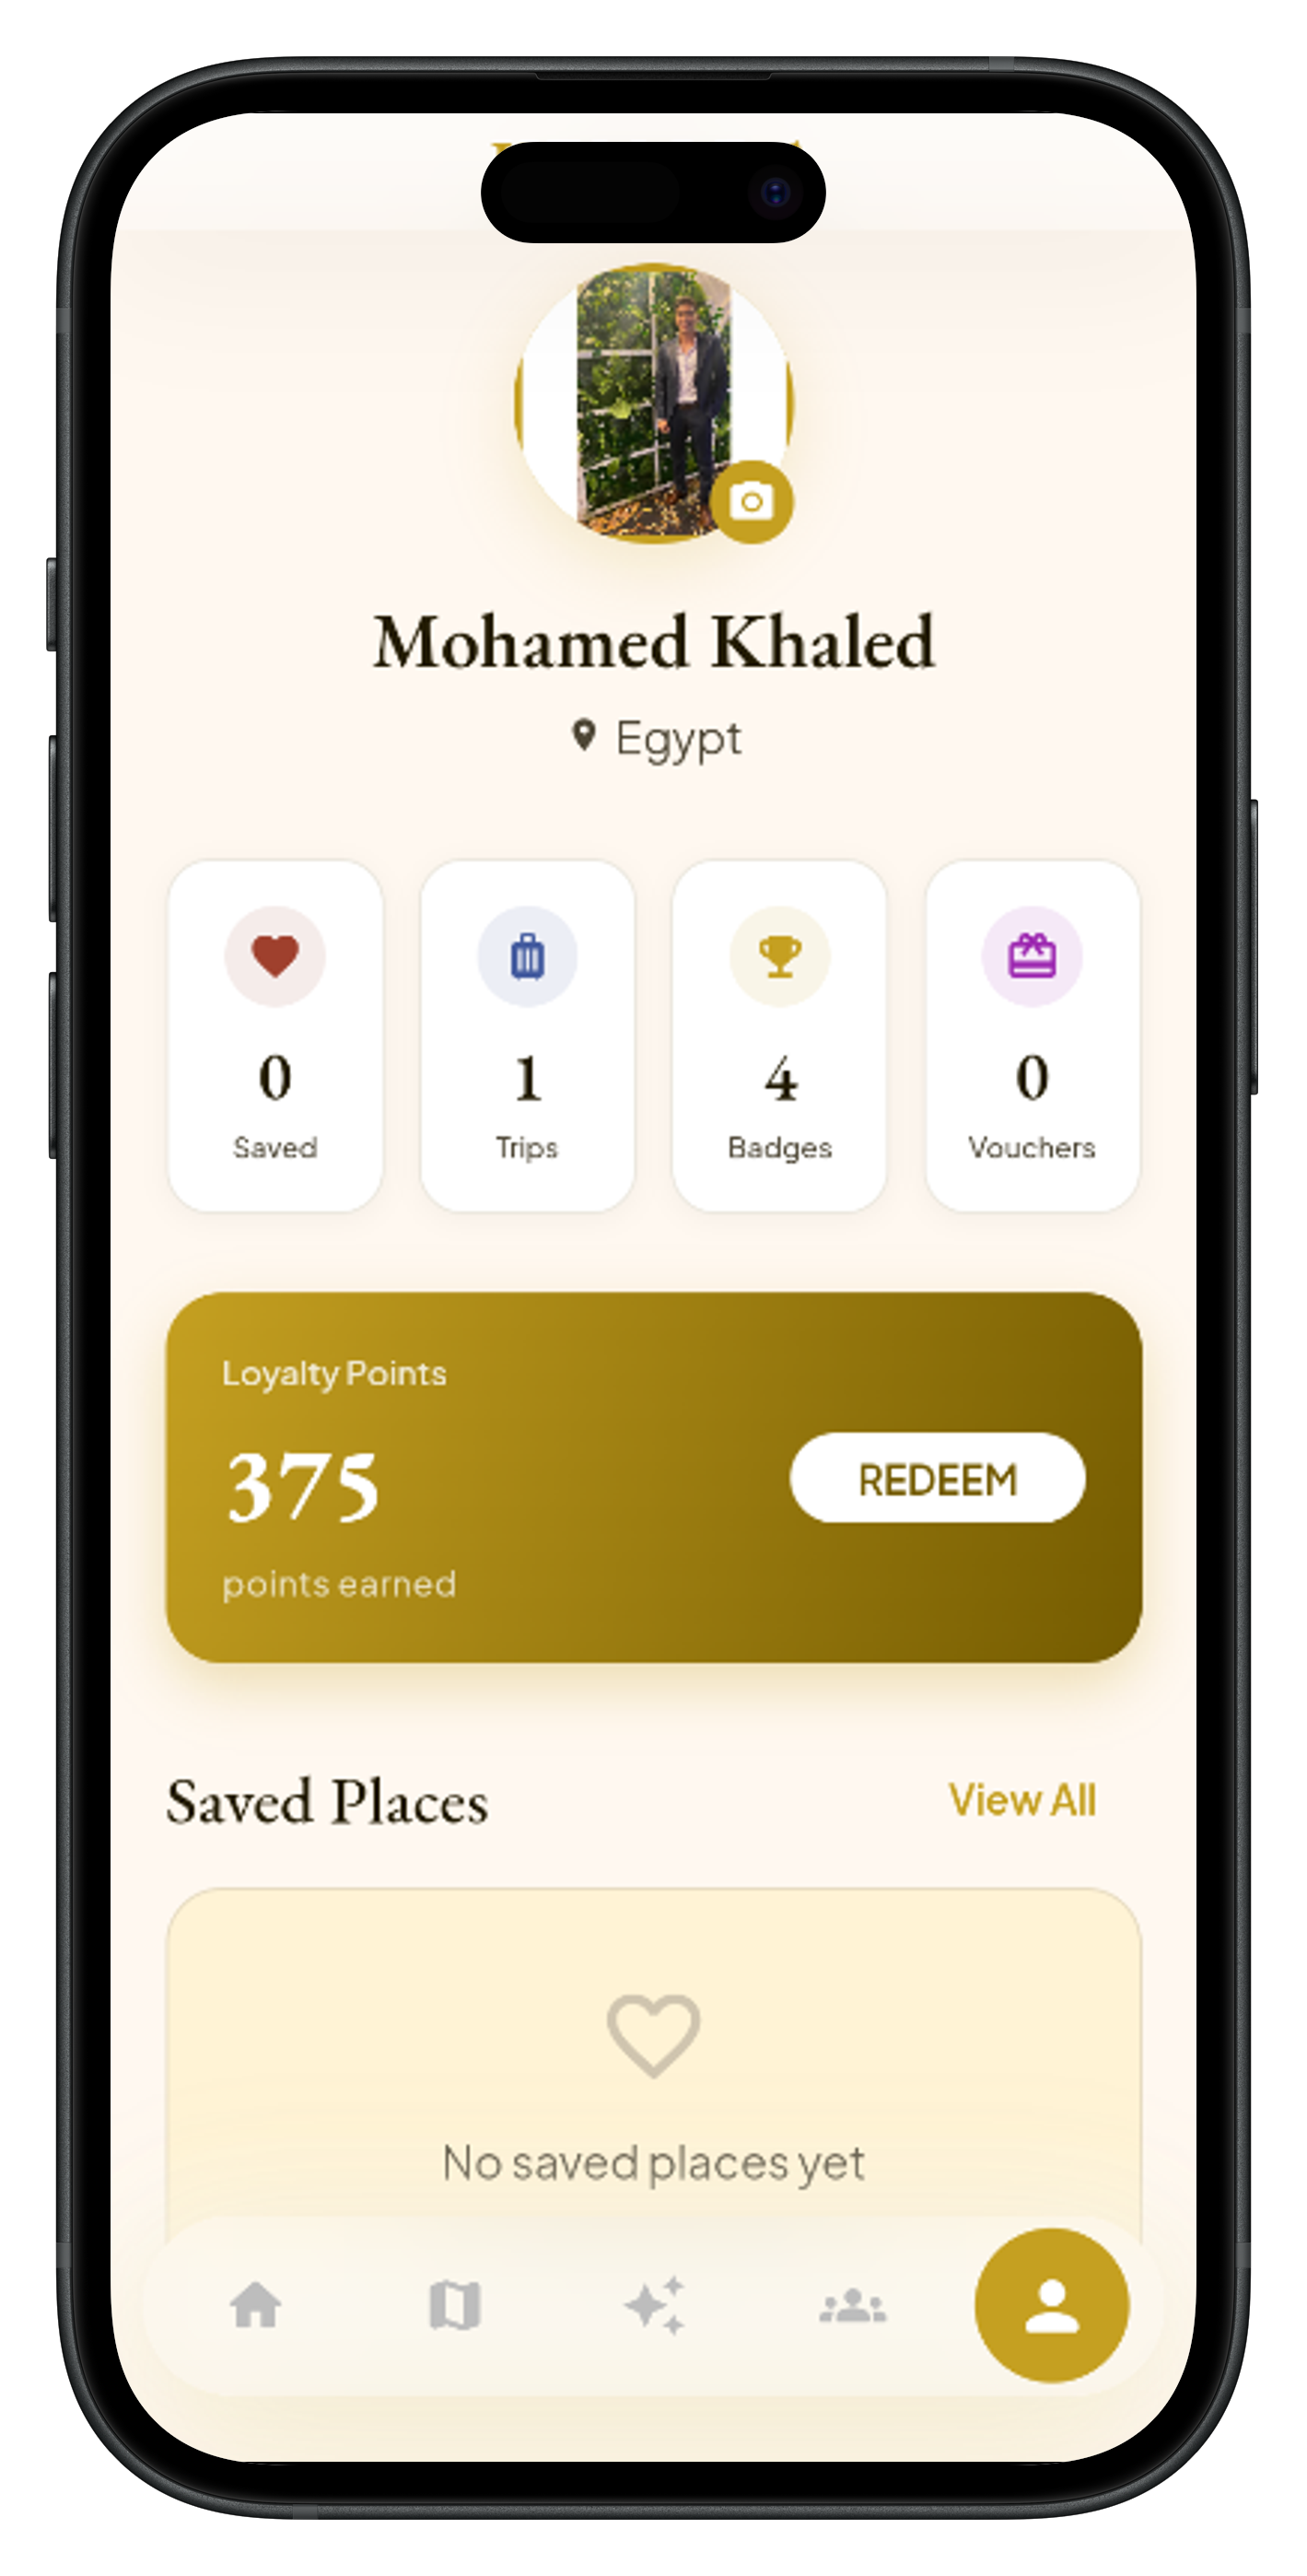
\includegraphics[width=\linewidth]{figures/profile.png}
        \caption{User Profile Screen}
        \label{fig:profile}
    \end{minipage}\hfill
    \begin{minipage}[t]{0.45\textwidth}
        \centering
        \vspace{0pt}
        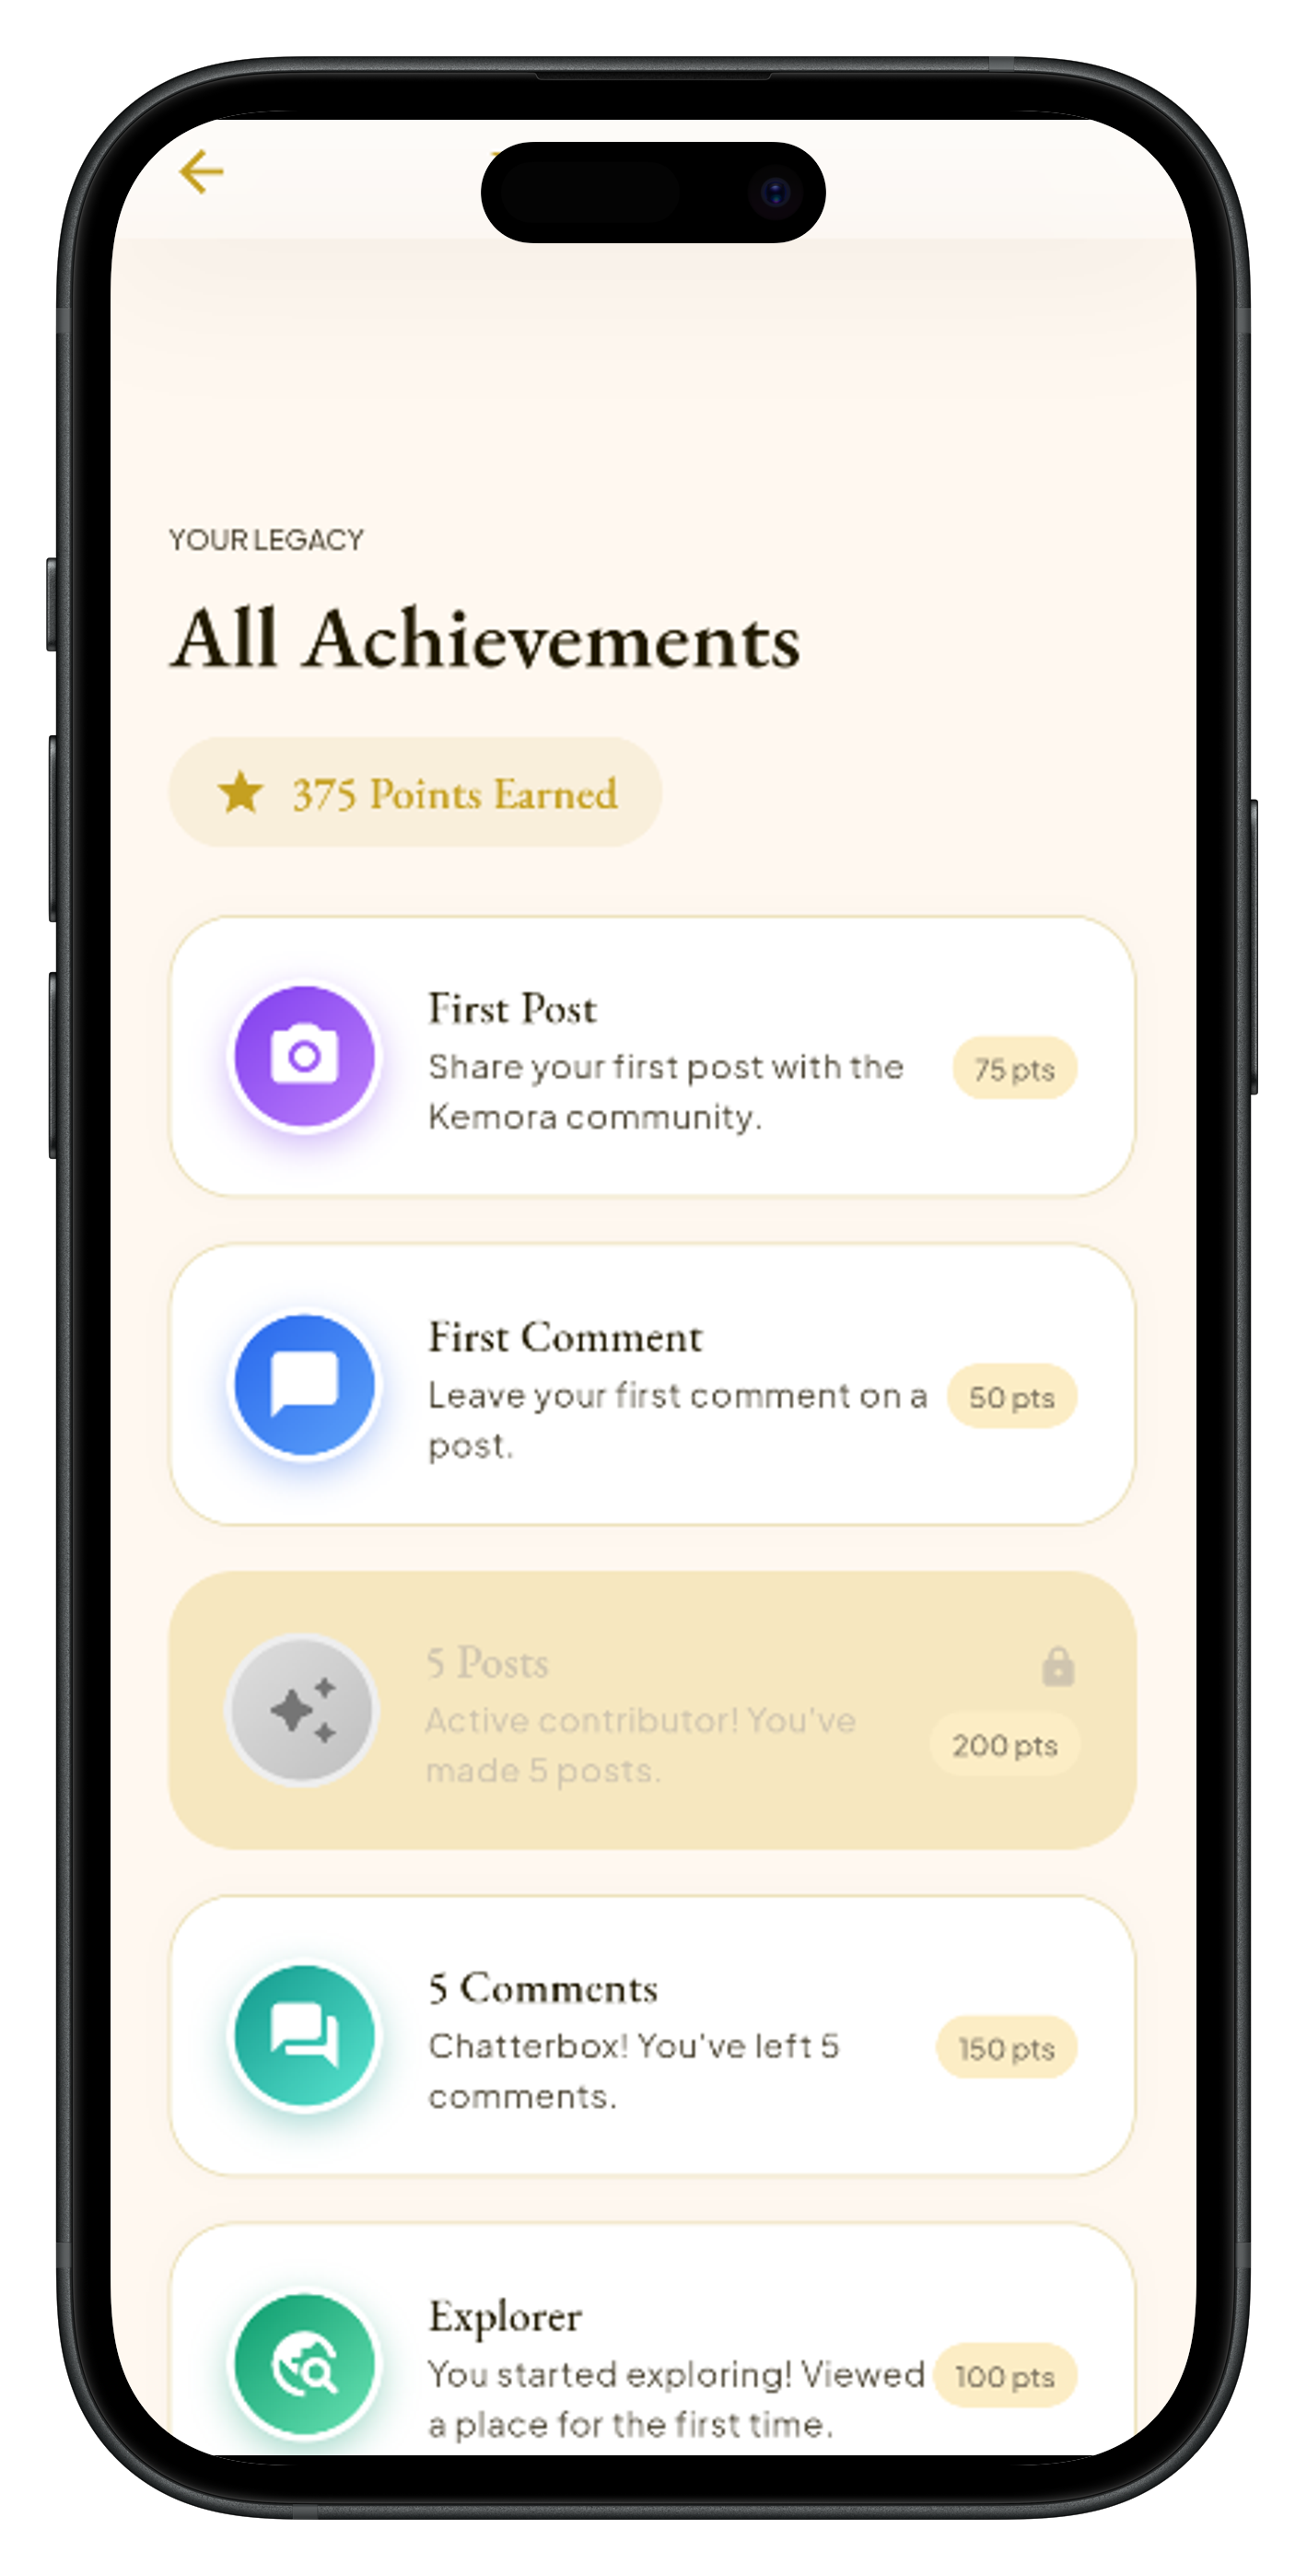
\includegraphics[width=\linewidth]{figures/badges.png}
        \caption{Gamification \& Badges Screen}
        \label{fig:badges}
    \end{minipage}
\end{figure}

\subsection{Offline-First Mobile Sync Strategy}
To provide a seamless user experience even in unreliable network conditions, Kemora employs an offline-first mobile sync strategy. Data fetched from the backend is aggressively cached using local embedded databases like SQLite and Hive. More importantly, when a user performs a data mutation---such as creating a trip, liking a post, or adding a comment---while offline, the action is not discarded. Instead, these mutations are serialized and appended to a local pending operations queue managed by SQLite/Hive. A background synchronization service periodically monitors network connectivity; upon detecting a stable connection, it flushes the queue, sequentially applying the pending mutations to the remote backend. This approach ensures high availability and consistency without compromising the responsiveness of the mobile frontend.
